\documentclass[twoside]{book}

% Packages required by doxygen
\usepackage{fixltx2e}
\usepackage{calc}
\usepackage{doxygen}
\usepackage[export]{adjustbox} % also loads graphicx
\usepackage{graphicx}
\usepackage[utf8]{inputenc}
\usepackage{makeidx}
\usepackage{multicol}
\usepackage{multirow}
\PassOptionsToPackage{warn}{textcomp}
\usepackage{textcomp}
\usepackage[nointegrals]{wasysym}
\usepackage[table]{xcolor}

% Font selection
\usepackage[T1]{fontenc}
\usepackage[scaled=.90]{helvet}
\usepackage{courier}
\usepackage{amssymb}
\usepackage{sectsty}
\renewcommand{\familydefault}{\sfdefault}
\allsectionsfont{%
  \fontseries{bc}\selectfont%
  \color{darkgray}%
}
\renewcommand{\DoxyLabelFont}{%
  \fontseries{bc}\selectfont%
  \color{darkgray}%
}
\newcommand{\+}{\discretionary{\mbox{\scriptsize$\hookleftarrow$}}{}{}}

% Page & text layout
\usepackage{geometry}
\geometry{%
  a4paper,%
  top=2.5cm,%
  bottom=2.5cm,%
  left=2.5cm,%
  right=2.5cm%
}
\tolerance=750
\hfuzz=15pt
\hbadness=750
\setlength{\emergencystretch}{15pt}
\setlength{\parindent}{0cm}
\setlength{\parskip}{3ex plus 2ex minus 2ex}
\makeatletter
\renewcommand{\paragraph}{%
  \@startsection{paragraph}{4}{0ex}{-1.0ex}{1.0ex}{%
    \normalfont\normalsize\bfseries\SS@parafont%
  }%
}
\renewcommand{\subparagraph}{%
  \@startsection{subparagraph}{5}{0ex}{-1.0ex}{1.0ex}{%
    \normalfont\normalsize\bfseries\SS@subparafont%
  }%
}
\makeatother

% Headers & footers
\usepackage{fancyhdr}
\pagestyle{fancyplain}
\fancyhead[LE]{\fancyplain{}{\bfseries\thepage}}
\fancyhead[CE]{\fancyplain{}{}}
\fancyhead[RE]{\fancyplain{}{\bfseries\leftmark}}
\fancyhead[LO]{\fancyplain{}{\bfseries\rightmark}}
\fancyhead[CO]{\fancyplain{}{}}
\fancyhead[RO]{\fancyplain{}{\bfseries\thepage}}
\fancyfoot[LE]{\fancyplain{}{}}
\fancyfoot[CE]{\fancyplain{}{}}
\fancyfoot[RE]{\fancyplain{}{\bfseries\scriptsize Generated by Doxygen }}
\fancyfoot[LO]{\fancyplain{}{\bfseries\scriptsize Generated by Doxygen }}
\fancyfoot[CO]{\fancyplain{}{}}
\fancyfoot[RO]{\fancyplain{}{}}
\renewcommand{\footrulewidth}{0.4pt}
\renewcommand{\chaptermark}[1]{%
  \markboth{#1}{}%
}
\renewcommand{\sectionmark}[1]{%
  \markright{\thesection\ #1}%
}

% Indices & bibliography
\usepackage{natbib}
\usepackage[titles]{tocloft}
\setcounter{tocdepth}{3}
\setcounter{secnumdepth}{5}
\makeindex

% Hyperlinks (required, but should be loaded last)
\usepackage{ifpdf}
\ifpdf
  \usepackage[pdftex,pagebackref=true]{hyperref}
\else
  \usepackage[ps2pdf,pagebackref=true]{hyperref}
\fi
\hypersetup{%
  colorlinks=true,%
  linkcolor=blue,%
  citecolor=blue,%
  unicode%
}

% Custom commands
\newcommand{\clearemptydoublepage}{%
  \newpage{\pagestyle{empty}\cleardoublepage}%
}

\usepackage{caption}
\captionsetup{labelsep=space,justification=centering,font={bf},singlelinecheck=off,skip=4pt,position=top}

%===== C O N T E N T S =====

\begin{document}

% Titlepage & ToC
\hypersetup{pageanchor=false,
             bookmarksnumbered=true,
             pdfencoding=unicode
            }
\pagenumbering{alph}
\begin{titlepage}
\vspace*{7cm}
\begin{center}%
{\Large u\+Boy (micro\+Boy) \\[1ex]\large 0.\+1 }\\
\vspace*{1cm}
{\large Generated by Doxygen 1.8.13}\\
\end{center}
\end{titlepage}
\clearemptydoublepage
\pagenumbering{roman}
\tableofcontents
\clearemptydoublepage
\pagenumbering{arabic}
\hypersetup{pageanchor=true}

%--- Begin generated contents ---
\chapter{File Index}
\section{File List}
Here is a list of all documented files with brief descriptions\+:\begin{DoxyCompactList}
\item\contentsline{section}{include/{\bfseries cpu.\+h} }{\pageref{cpu_8h}}{}
\item\contentsline{section}{include/{\bfseries debug.\+h} }{\pageref{debug_8h}}{}
\item\contentsline{section}{include/\hyperlink{instructions_8h}{instructions.\+h} \\*A set of reusable instructions that are called by the opcode functions }{\pageref{instructions_8h}}{}
\item\contentsline{section}{include/\hyperlink{memory_8h}{memory.\+h} \\*Representation of the Game Boy\textquotesingle{}s memory model and operations to read and write to this memory }{\pageref{memory_8h}}{}
\item\contentsline{section}{include/{\bfseries ppu.\+h} }{\pageref{ppu_8h}}{}
\item\contentsline{section}{include/\hyperlink{state_8h}{state.\+h} \\*Representation of the state of the emulator (registers, C\+PU mode, flags) and a set of utility functions }{\pageref{state_8h}}{}
\end{DoxyCompactList}

\chapter{File Documentation}
\hypertarget{instructions_8h}{}\section{include/instructions.h File Reference}
\label{instructions_8h}\index{include/instructions.\+h@{include/instructions.\+h}}


A set of reusable instructions that are called by the opcode functions.  


{\ttfamily \#include \char`\"{}memory.\+h\char`\"{}}\newline
{\ttfamily \#include \char`\"{}state.\+h\char`\"{}}\newline
Include dependency graph for instructions.\+h\+:\nopagebreak
\begin{figure}[H]
\begin{center}
\leavevmode
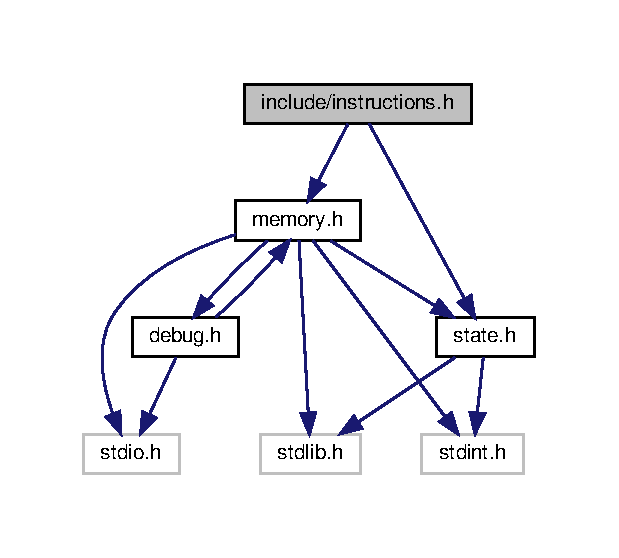
\includegraphics[width=297pt]{instructions_8h__incl}
\end{center}
\end{figure}
This graph shows which files directly or indirectly include this file\+:\nopagebreak
\begin{figure}[H]
\begin{center}
\leavevmode
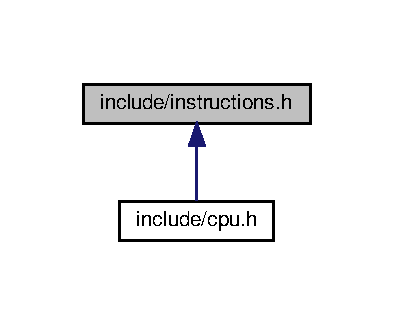
\includegraphics[width=189pt]{instructions_8h__dep__incl}
\end{center}
\end{figure}
\subsection*{Functions}
\begin{DoxyCompactItemize}
\item 
void \hyperlink{instructions_8h_a53810b54e095653d325cc4a05ab33ed5}{Instruction\+\_\+\+A\+D\+D\+\_\+N} (uint8\+\_\+t n)
\begin{DoxyCompactList}\small\item\em Add unsigned 8-\/bit constant to register A. \end{DoxyCompactList}\item 
void \hyperlink{instructions_8h_aecd21031952e16551c4f1f1f40d9d3f7}{Instruction\+\_\+\+A\+D\+C\+\_\+N} (uint8\+\_\+t n)
\begin{DoxyCompactList}\small\item\em Add unsigned 8-\/bit constant and carry flag to register A. \end{DoxyCompactList}\item 
void \hyperlink{instructions_8h_a23af2d18c12397dd80baa0108966fb81}{Instruction\+\_\+\+S\+U\+B\+\_\+N} (uint8\+\_\+t n)
\begin{DoxyCompactList}\small\item\em Subtract unsigned 8-\/bit constant from register A. \end{DoxyCompactList}\item 
void \hyperlink{instructions_8h_adb0e3134fb0874a20dd9fbe27431165d}{Instruction\+\_\+\+S\+B\+C\+\_\+N} (uint8\+\_\+t n)
\begin{DoxyCompactList}\small\item\em Subtract unsigned 8-\/bit constant and carry flag from register A. \end{DoxyCompactList}\item 
void \hyperlink{instructions_8h_a5cf6516a2fe8d40c4bad2014435a986b}{Instruction\+\_\+\+A\+N\+D\+\_\+N} (uint8\+\_\+t n)
\begin{DoxyCompactList}\small\item\em Apply bitwise A\+ND operation on register A and an unsigned 8-\/bit constant. \end{DoxyCompactList}\item 
void \hyperlink{instructions_8h_ad82fd3f5e54acda061336b4b7d24796b}{Instruction\+\_\+\+O\+R\+\_\+N} (uint8\+\_\+t n)
\begin{DoxyCompactList}\small\item\em Apply bitwise OR operation on register A and an unsigned 8-\/bit constant. \end{DoxyCompactList}\item 
void \hyperlink{instructions_8h_a16a374675ed22b20f8234e533a820ffd}{Instruction\+\_\+\+X\+O\+R\+\_\+N} (uint8\+\_\+t n)
\begin{DoxyCompactList}\small\item\em Apply bitwise X\+OR operation on register A and an unsigned 8-\/bit constant. \end{DoxyCompactList}\item 
void \hyperlink{instructions_8h_a283ba06d0e951780848b47c248c32c28}{Instruction\+\_\+\+C\+P\+\_\+N} (uint8\+\_\+t n)
\begin{DoxyCompactList}\small\item\em Compare the value in register A with an unsigned 8-\/bit constant. Essentially, this function subtracts the constant from the register value, sets the flags accordingly and throws away the result of the substraction. \end{DoxyCompactList}\item 
void \hyperlink{instructions_8h_afd959af095696914d74c68e9a95295f7}{Instruction\+\_\+\+I\+N\+C\+\_\+N} (uint8\+\_\+t $\ast$r)
\begin{DoxyCompactList}\small\item\em Increment the value in a given register. \end{DoxyCompactList}\item 
void \hyperlink{instructions_8h_acc69a782eb9f5a070a62013abde81fa8}{Instruction\+\_\+\+D\+E\+C\+\_\+N} (uint8\+\_\+t $\ast$r)
\begin{DoxyCompactList}\small\item\em Decrement the value in a given register. \end{DoxyCompactList}\item 
void \hyperlink{instructions_8h_adc5ceb5389c6a4caa364b261d714536f}{Instruction\+\_\+\+A\+D\+D\+\_\+\+H\+L\+\_\+\+NN} (uint16\+\_\+t nn)
\begin{DoxyCompactList}\small\item\em Add an unsigned 16-\/bit constant to register HL. \end{DoxyCompactList}\item 
void \hyperlink{instructions_8h_a2364a4fdad07ba894b911061b1a8cb5c}{Instruction\+\_\+\+C\+A\+L\+L\+\_\+\+NN} (uint16\+\_\+t nn)
\begin{DoxyCompactList}\small\item\em Push the current program counter on the stack and set the program counter to an unsigned 16-\/bit constant (address). \end{DoxyCompactList}\item 
void \hyperlink{instructions_8h_a27f54c92e32ca954fc39a52f557c1ccd}{Instruction\+\_\+\+R\+S\+T\+\_\+N} (uint8\+\_\+t n)
\begin{DoxyCompactList}\small\item\em Push the current program counter on the stack and set the program counter to an unsigned 8-\/bit constant (address). \end{DoxyCompactList}\item 
\mbox{\Hypertarget{instructions_8h_a5cb5475b8784a50018e7271557c2e868}\label{instructions_8h_a5cb5475b8784a50018e7271557c2e868}} 
void \hyperlink{instructions_8h_a5cb5475b8784a50018e7271557c2e868}{Instruction\+\_\+\+R\+ET} (void)
\begin{DoxyCompactList}\small\item\em Pop two bytes from the stack and set the program counter to the 16-\/bit address these bytes form. \end{DoxyCompactList}\item 
void \hyperlink{instructions_8h_a013e0f73f245066aca203b657fad414c}{Instruction\+\_\+\+S\+E\+T\+\_\+\+N\+\_\+R} (uint8\+\_\+t n, uint8\+\_\+t $\ast$r)
\begin{DoxyCompactList}\small\item\em Set the nth bit of a given register. \end{DoxyCompactList}\item 
void \hyperlink{instructions_8h_a42a033ef02c7a4f9fc4e4de62610c538}{Instruction\+\_\+\+S\+E\+T\+\_\+\+N\+\_\+M} (uint8\+\_\+t n, uint16\+\_\+t m)
\begin{DoxyCompactList}\small\item\em Set the nth bit of a byte in memory. \end{DoxyCompactList}\item 
void \hyperlink{instructions_8h_a4871f18b19b6ebb9add69b5a1ddb5d37}{Instruction\+\_\+\+R\+E\+S\+\_\+\+N\+\_\+R} (uint8\+\_\+t n, uint8\+\_\+t $\ast$r)
\begin{DoxyCompactList}\small\item\em Reset the nth bit of a given register. \end{DoxyCompactList}\item 
void \hyperlink{instructions_8h_afae47874f6a2e9407092d2b7002f7d7e}{Instruction\+\_\+\+R\+E\+S\+\_\+\+N\+\_\+M} (uint8\+\_\+t n, uint16\+\_\+t m)
\begin{DoxyCompactList}\small\item\em Reset the nth bit of a byte in memory. \end{DoxyCompactList}\item 
void \hyperlink{instructions_8h_a50f25c42aae5d9f8423e3214e949e2ce}{Instruction\+\_\+\+B\+I\+T\+\_\+\+N\+\_\+R} (uint8\+\_\+t n, uint8\+\_\+t r)
\begin{DoxyCompactList}\small\item\em Test the nth bit of an unsigned 8-\/bit register (set flags accordingly). \end{DoxyCompactList}\item 
void \hyperlink{instructions_8h_a31d1bb1052756ef7694f58da1a0ce622}{Instruction\+\_\+\+B\+I\+T\+\_\+\+N\+\_\+M} (uint8\+\_\+t n, uint16\+\_\+t m)
\begin{DoxyCompactList}\small\item\em Test the nth bit of a byte in memory (set flags accordingly). \end{DoxyCompactList}\item 
void \hyperlink{instructions_8h_a4712224a421ff429dbbda237d505493b}{Instruction\+\_\+\+S\+W\+A\+P\+\_\+\+N\+\_\+R} (uint8\+\_\+t $\ast$r)
\begin{DoxyCompactList}\small\item\em Swap the order of the two nibbles in an unsigned 8-\/bit register. \end{DoxyCompactList}\item 
void \hyperlink{instructions_8h_aeed3d4f7f6615285a147e71704ee8f2d}{Instruction\+\_\+\+S\+W\+A\+P\+\_\+\+N\+\_\+M} (uint16\+\_\+t m)
\begin{DoxyCompactList}\small\item\em Swap the order of the two nibbles of a byte in memory. \end{DoxyCompactList}\item 
void \hyperlink{instructions_8h_abe04d911de4baebc972d22d0e21d5d9c}{Instruction\+\_\+\+S\+R\+L\+\_\+\+N\+\_\+R} (uint8\+\_\+t $\ast$r)
\begin{DoxyCompactList}\small\item\em Shift an unsigned 8-\/bit register to the right. The L\+SB is pushed into the carry flag and the M\+SB is set to 0. \end{DoxyCompactList}\item 
void \hyperlink{instructions_8h_a58d942db75699e8e6849f89e51794adb}{Instruction\+\_\+\+S\+R\+L\+\_\+\+N\+\_\+M} (uint16\+\_\+t m)
\begin{DoxyCompactList}\small\item\em Shift a byte in memory to the right. The L\+SB is pushed into the carry flag and the M\+SB is set to 0. \end{DoxyCompactList}\item 
void \hyperlink{instructions_8h_a11968a23b64c558ca28d225c9a9d3e66}{Instruction\+\_\+\+S\+L\+A\+\_\+\+N\+\_\+R} (uint8\+\_\+t $\ast$r)
\begin{DoxyCompactList}\small\item\em Shift an unsigned 8-\/bit register to the left. The M\+SB is pushed into the carry flag and the L\+SB is set to 0. \end{DoxyCompactList}\item 
void \hyperlink{instructions_8h_a90e53de8050b506e214c5ffba1907700}{Instruction\+\_\+\+S\+L\+A\+\_\+\+N\+\_\+M} (uint16\+\_\+t m)
\begin{DoxyCompactList}\small\item\em Shift a byte in memory to the left. The M\+SB is pushed into the carry flag and the L\+SB is set to 0. \end{DoxyCompactList}\item 
void \hyperlink{instructions_8h_af68fa257074f039dabc5458327cd818c}{Instruction\+\_\+\+S\+R\+A\+\_\+\+N\+\_\+R} (uint8\+\_\+t $\ast$r)
\begin{DoxyCompactList}\small\item\em Shift an unsigned 8-\/bit register to the right. The L\+SB is pushed into the carry flag and the M\+SB remains the value it had before the shift. \end{DoxyCompactList}\item 
void \hyperlink{instructions_8h_ac12ec42750fabe5740636cea3b33b865}{Instruction\+\_\+\+S\+R\+A\+\_\+\+N\+\_\+M} (uint16\+\_\+t m)
\begin{DoxyCompactList}\small\item\em Shift a byte in memory to the right. The L\+SB is pushed into the carry flag and the M\+SB remains the value it has before the shift. \end{DoxyCompactList}\item 
void \hyperlink{instructions_8h_a37420f7031217dc8504d3df5230e7e6b}{Instruction\+\_\+\+R\+L\+\_\+\+N\+\_\+R} (uint8\+\_\+t $\ast$r)
\begin{DoxyCompactList}\small\item\em Rotate an unsigned 8-\/bit register to the left through the carry flag. \end{DoxyCompactList}\item 
void \hyperlink{instructions_8h_a5901146f06a4aca964560e38d9e6431d}{Instruction\+\_\+\+R\+L\+\_\+\+N\+\_\+M} (uint16\+\_\+t m)
\begin{DoxyCompactList}\small\item\em Rotate a byte in memory to the left through the carry flag. \end{DoxyCompactList}\item 
void \hyperlink{instructions_8h_a8409550d3a3c830689806133a48894b6}{Instruction\+\_\+\+R\+R\+\_\+\+N\+\_\+R} (uint8\+\_\+t $\ast$r)
\begin{DoxyCompactList}\small\item\em Rotate an unsigned 8-\/bit register to the right through the carry flag. \end{DoxyCompactList}\item 
void \hyperlink{instructions_8h_a591febd710ace13bd8c988f91b07fd3c}{Instruction\+\_\+\+R\+R\+\_\+\+N\+\_\+M} (uint16\+\_\+t m)
\begin{DoxyCompactList}\small\item\em Rotate a byte in memory to the right through the carry flag. \end{DoxyCompactList}\item 
void \hyperlink{instructions_8h_a5d8d8838f46f9a451f6e86cfd8a493e3}{Instruction\+\_\+\+R\+L\+C\+\_\+\+N\+\_\+R} (uint8\+\_\+t $\ast$r)
\begin{DoxyCompactList}\small\item\em Rotate an unsigned 8-\/bit register to the left and store the former M\+SB in the carry flag. \end{DoxyCompactList}\item 
void \hyperlink{instructions_8h_a82407a01bfcdd76a41f29fe7c65e4b0c}{Instruction\+\_\+\+R\+L\+C\+\_\+\+N\+\_\+M} (uint16\+\_\+t m)
\begin{DoxyCompactList}\small\item\em Rotate a byte in memory to the left and store the former M\+SB in the carry flag. \end{DoxyCompactList}\item 
void \hyperlink{instructions_8h_acbebe19a94499a25f7565d30968a1c10}{Instruction\+\_\+\+R\+R\+C\+\_\+\+N\+\_\+R} (uint8\+\_\+t $\ast$r)
\begin{DoxyCompactList}\small\item\em Rotate an unsigned 8-\/bit register to the right and store the former L\+SB in the carry flag. \end{DoxyCompactList}\item 
void \hyperlink{instructions_8h_a2aec819714543a7b7ccc02dc76943462}{Instruction\+\_\+\+R\+R\+C\+\_\+\+N\+\_\+M} (uint16\+\_\+t m)
\begin{DoxyCompactList}\small\item\em Rotate a byte in memory to the right and store the former L\+SB in the carry flag. \end{DoxyCompactList}\end{DoxyCompactItemize}


\subsection{Detailed Description}
A set of reusable instructions that are called by the opcode functions. 

\begin{DoxyAuthor}{Author}
tbnbooij 
\end{DoxyAuthor}
\begin{DoxyDate}{Date}
2018-\/08-\/13 
\end{DoxyDate}


\subsection{Function Documentation}
\mbox{\Hypertarget{instructions_8h_aecd21031952e16551c4f1f1f40d9d3f7}\label{instructions_8h_aecd21031952e16551c4f1f1f40d9d3f7}} 
\index{instructions.\+h@{instructions.\+h}!Instruction\+\_\+\+A\+D\+C\+\_\+N@{Instruction\+\_\+\+A\+D\+C\+\_\+N}}
\index{Instruction\+\_\+\+A\+D\+C\+\_\+N@{Instruction\+\_\+\+A\+D\+C\+\_\+N}!instructions.\+h@{instructions.\+h}}
\subsubsection{\texorpdfstring{Instruction\+\_\+\+A\+D\+C\+\_\+\+N()}{Instruction\_ADC\_N()}}
{\footnotesize\ttfamily void Instruction\+\_\+\+A\+D\+C\+\_\+N (\begin{DoxyParamCaption}\item[{uint8\+\_\+t}]{n }\end{DoxyParamCaption})}



Add unsigned 8-\/bit constant and carry flag to register A. 


\begin{DoxyParams}{Parameters}
{\em n} & Unsigned 8-\/bit constant \\
\hline
\end{DoxyParams}
\mbox{\Hypertarget{instructions_8h_adc5ceb5389c6a4caa364b261d714536f}\label{instructions_8h_adc5ceb5389c6a4caa364b261d714536f}} 
\index{instructions.\+h@{instructions.\+h}!Instruction\+\_\+\+A\+D\+D\+\_\+\+H\+L\+\_\+\+NN@{Instruction\+\_\+\+A\+D\+D\+\_\+\+H\+L\+\_\+\+NN}}
\index{Instruction\+\_\+\+A\+D\+D\+\_\+\+H\+L\+\_\+\+NN@{Instruction\+\_\+\+A\+D\+D\+\_\+\+H\+L\+\_\+\+NN}!instructions.\+h@{instructions.\+h}}
\subsubsection{\texorpdfstring{Instruction\+\_\+\+A\+D\+D\+\_\+\+H\+L\+\_\+\+N\+N()}{Instruction\_ADD\_HL\_NN()}}
{\footnotesize\ttfamily void Instruction\+\_\+\+A\+D\+D\+\_\+\+H\+L\+\_\+\+NN (\begin{DoxyParamCaption}\item[{uint16\+\_\+t}]{nn }\end{DoxyParamCaption})}



Add an unsigned 16-\/bit constant to register HL. 


\begin{DoxyParams}{Parameters}
{\em nn} & Unsigned 16-\/bit constant \\
\hline
\end{DoxyParams}
\mbox{\Hypertarget{instructions_8h_a53810b54e095653d325cc4a05ab33ed5}\label{instructions_8h_a53810b54e095653d325cc4a05ab33ed5}} 
\index{instructions.\+h@{instructions.\+h}!Instruction\+\_\+\+A\+D\+D\+\_\+N@{Instruction\+\_\+\+A\+D\+D\+\_\+N}}
\index{Instruction\+\_\+\+A\+D\+D\+\_\+N@{Instruction\+\_\+\+A\+D\+D\+\_\+N}!instructions.\+h@{instructions.\+h}}
\subsubsection{\texorpdfstring{Instruction\+\_\+\+A\+D\+D\+\_\+\+N()}{Instruction\_ADD\_N()}}
{\footnotesize\ttfamily void Instruction\+\_\+\+A\+D\+D\+\_\+N (\begin{DoxyParamCaption}\item[{uint8\+\_\+t}]{n }\end{DoxyParamCaption})}



Add unsigned 8-\/bit constant to register A. 


\begin{DoxyParams}{Parameters}
{\em n} & Unsigned 8-\/bit constant \\
\hline
\end{DoxyParams}
\mbox{\Hypertarget{instructions_8h_a5cf6516a2fe8d40c4bad2014435a986b}\label{instructions_8h_a5cf6516a2fe8d40c4bad2014435a986b}} 
\index{instructions.\+h@{instructions.\+h}!Instruction\+\_\+\+A\+N\+D\+\_\+N@{Instruction\+\_\+\+A\+N\+D\+\_\+N}}
\index{Instruction\+\_\+\+A\+N\+D\+\_\+N@{Instruction\+\_\+\+A\+N\+D\+\_\+N}!instructions.\+h@{instructions.\+h}}
\subsubsection{\texorpdfstring{Instruction\+\_\+\+A\+N\+D\+\_\+\+N()}{Instruction\_AND\_N()}}
{\footnotesize\ttfamily void Instruction\+\_\+\+A\+N\+D\+\_\+N (\begin{DoxyParamCaption}\item[{uint8\+\_\+t}]{n }\end{DoxyParamCaption})}



Apply bitwise A\+ND operation on register A and an unsigned 8-\/bit constant. 


\begin{DoxyParams}{Parameters}
{\em n} & Unsigned 8-\/bit constant \\
\hline
\end{DoxyParams}
\mbox{\Hypertarget{instructions_8h_a31d1bb1052756ef7694f58da1a0ce622}\label{instructions_8h_a31d1bb1052756ef7694f58da1a0ce622}} 
\index{instructions.\+h@{instructions.\+h}!Instruction\+\_\+\+B\+I\+T\+\_\+\+N\+\_\+M@{Instruction\+\_\+\+B\+I\+T\+\_\+\+N\+\_\+M}}
\index{Instruction\+\_\+\+B\+I\+T\+\_\+\+N\+\_\+M@{Instruction\+\_\+\+B\+I\+T\+\_\+\+N\+\_\+M}!instructions.\+h@{instructions.\+h}}
\subsubsection{\texorpdfstring{Instruction\+\_\+\+B\+I\+T\+\_\+\+N\+\_\+\+M()}{Instruction\_BIT\_N\_M()}}
{\footnotesize\ttfamily void Instruction\+\_\+\+B\+I\+T\+\_\+\+N\+\_\+M (\begin{DoxyParamCaption}\item[{uint8\+\_\+t}]{n,  }\item[{uint16\+\_\+t}]{m }\end{DoxyParamCaption})}



Test the nth bit of a byte in memory (set flags accordingly). 


\begin{DoxyParams}{Parameters}
{\em n} & The index of the bit that will be tested (little-\/endian, indexed from 0) \\
\hline
{\em m} & The 16-\/bit address of the tested byte \\
\hline
\end{DoxyParams}
\mbox{\Hypertarget{instructions_8h_a50f25c42aae5d9f8423e3214e949e2ce}\label{instructions_8h_a50f25c42aae5d9f8423e3214e949e2ce}} 
\index{instructions.\+h@{instructions.\+h}!Instruction\+\_\+\+B\+I\+T\+\_\+\+N\+\_\+R@{Instruction\+\_\+\+B\+I\+T\+\_\+\+N\+\_\+R}}
\index{Instruction\+\_\+\+B\+I\+T\+\_\+\+N\+\_\+R@{Instruction\+\_\+\+B\+I\+T\+\_\+\+N\+\_\+R}!instructions.\+h@{instructions.\+h}}
\subsubsection{\texorpdfstring{Instruction\+\_\+\+B\+I\+T\+\_\+\+N\+\_\+\+R()}{Instruction\_BIT\_N\_R()}}
{\footnotesize\ttfamily void Instruction\+\_\+\+B\+I\+T\+\_\+\+N\+\_\+R (\begin{DoxyParamCaption}\item[{uint8\+\_\+t}]{n,  }\item[{uint8\+\_\+t}]{r }\end{DoxyParamCaption})}



Test the nth bit of an unsigned 8-\/bit register (set flags accordingly). 


\begin{DoxyParams}{Parameters}
{\em n} & The index of the bit that will be tested (little-\/endian, indexed from 0) \\
\hline
{\em r} & The value in an unsigned 8-\/bit register \\
\hline
\end{DoxyParams}
\mbox{\Hypertarget{instructions_8h_a2364a4fdad07ba894b911061b1a8cb5c}\label{instructions_8h_a2364a4fdad07ba894b911061b1a8cb5c}} 
\index{instructions.\+h@{instructions.\+h}!Instruction\+\_\+\+C\+A\+L\+L\+\_\+\+NN@{Instruction\+\_\+\+C\+A\+L\+L\+\_\+\+NN}}
\index{Instruction\+\_\+\+C\+A\+L\+L\+\_\+\+NN@{Instruction\+\_\+\+C\+A\+L\+L\+\_\+\+NN}!instructions.\+h@{instructions.\+h}}
\subsubsection{\texorpdfstring{Instruction\+\_\+\+C\+A\+L\+L\+\_\+\+N\+N()}{Instruction\_CALL\_NN()}}
{\footnotesize\ttfamily void Instruction\+\_\+\+C\+A\+L\+L\+\_\+\+NN (\begin{DoxyParamCaption}\item[{uint16\+\_\+t}]{nn }\end{DoxyParamCaption})}



Push the current program counter on the stack and set the program counter to an unsigned 16-\/bit constant (address). 


\begin{DoxyParams}{Parameters}
{\em nn} & 16-\/bit address the PC is set to \\
\hline
\end{DoxyParams}
\mbox{\Hypertarget{instructions_8h_a283ba06d0e951780848b47c248c32c28}\label{instructions_8h_a283ba06d0e951780848b47c248c32c28}} 
\index{instructions.\+h@{instructions.\+h}!Instruction\+\_\+\+C\+P\+\_\+N@{Instruction\+\_\+\+C\+P\+\_\+N}}
\index{Instruction\+\_\+\+C\+P\+\_\+N@{Instruction\+\_\+\+C\+P\+\_\+N}!instructions.\+h@{instructions.\+h}}
\subsubsection{\texorpdfstring{Instruction\+\_\+\+C\+P\+\_\+\+N()}{Instruction\_CP\_N()}}
{\footnotesize\ttfamily void Instruction\+\_\+\+C\+P\+\_\+N (\begin{DoxyParamCaption}\item[{uint8\+\_\+t}]{n }\end{DoxyParamCaption})}



Compare the value in register A with an unsigned 8-\/bit constant. Essentially, this function subtracts the constant from the register value, sets the flags accordingly and throws away the result of the substraction. 


\begin{DoxyParams}{Parameters}
{\em n} & Unsigned 8-\/bit constant \\
\hline
\end{DoxyParams}
\mbox{\Hypertarget{instructions_8h_acc69a782eb9f5a070a62013abde81fa8}\label{instructions_8h_acc69a782eb9f5a070a62013abde81fa8}} 
\index{instructions.\+h@{instructions.\+h}!Instruction\+\_\+\+D\+E\+C\+\_\+N@{Instruction\+\_\+\+D\+E\+C\+\_\+N}}
\index{Instruction\+\_\+\+D\+E\+C\+\_\+N@{Instruction\+\_\+\+D\+E\+C\+\_\+N}!instructions.\+h@{instructions.\+h}}
\subsubsection{\texorpdfstring{Instruction\+\_\+\+D\+E\+C\+\_\+\+N()}{Instruction\_DEC\_N()}}
{\footnotesize\ttfamily void Instruction\+\_\+\+D\+E\+C\+\_\+N (\begin{DoxyParamCaption}\item[{uint8\+\_\+t $\ast$}]{r }\end{DoxyParamCaption})}



Decrement the value in a given register. 


\begin{DoxyParams}{Parameters}
{\em $\ast$r} & Pointer to an unsigned 8-\/bit register \\
\hline
\end{DoxyParams}
\mbox{\Hypertarget{instructions_8h_afd959af095696914d74c68e9a95295f7}\label{instructions_8h_afd959af095696914d74c68e9a95295f7}} 
\index{instructions.\+h@{instructions.\+h}!Instruction\+\_\+\+I\+N\+C\+\_\+N@{Instruction\+\_\+\+I\+N\+C\+\_\+N}}
\index{Instruction\+\_\+\+I\+N\+C\+\_\+N@{Instruction\+\_\+\+I\+N\+C\+\_\+N}!instructions.\+h@{instructions.\+h}}
\subsubsection{\texorpdfstring{Instruction\+\_\+\+I\+N\+C\+\_\+\+N()}{Instruction\_INC\_N()}}
{\footnotesize\ttfamily void Instruction\+\_\+\+I\+N\+C\+\_\+N (\begin{DoxyParamCaption}\item[{uint8\+\_\+t $\ast$}]{r }\end{DoxyParamCaption})}



Increment the value in a given register. 


\begin{DoxyParams}{Parameters}
{\em $\ast$r} & Pointer to an unsigned 8-\/bit register \\
\hline
\end{DoxyParams}
\mbox{\Hypertarget{instructions_8h_ad82fd3f5e54acda061336b4b7d24796b}\label{instructions_8h_ad82fd3f5e54acda061336b4b7d24796b}} 
\index{instructions.\+h@{instructions.\+h}!Instruction\+\_\+\+O\+R\+\_\+N@{Instruction\+\_\+\+O\+R\+\_\+N}}
\index{Instruction\+\_\+\+O\+R\+\_\+N@{Instruction\+\_\+\+O\+R\+\_\+N}!instructions.\+h@{instructions.\+h}}
\subsubsection{\texorpdfstring{Instruction\+\_\+\+O\+R\+\_\+\+N()}{Instruction\_OR\_N()}}
{\footnotesize\ttfamily void Instruction\+\_\+\+O\+R\+\_\+N (\begin{DoxyParamCaption}\item[{uint8\+\_\+t}]{n }\end{DoxyParamCaption})}



Apply bitwise OR operation on register A and an unsigned 8-\/bit constant. 


\begin{DoxyParams}{Parameters}
{\em n} & Unsigned 8-\/bit constant \\
\hline
\end{DoxyParams}
\mbox{\Hypertarget{instructions_8h_afae47874f6a2e9407092d2b7002f7d7e}\label{instructions_8h_afae47874f6a2e9407092d2b7002f7d7e}} 
\index{instructions.\+h@{instructions.\+h}!Instruction\+\_\+\+R\+E\+S\+\_\+\+N\+\_\+M@{Instruction\+\_\+\+R\+E\+S\+\_\+\+N\+\_\+M}}
\index{Instruction\+\_\+\+R\+E\+S\+\_\+\+N\+\_\+M@{Instruction\+\_\+\+R\+E\+S\+\_\+\+N\+\_\+M}!instructions.\+h@{instructions.\+h}}
\subsubsection{\texorpdfstring{Instruction\+\_\+\+R\+E\+S\+\_\+\+N\+\_\+\+M()}{Instruction\_RES\_N\_M()}}
{\footnotesize\ttfamily void Instruction\+\_\+\+R\+E\+S\+\_\+\+N\+\_\+M (\begin{DoxyParamCaption}\item[{uint8\+\_\+t}]{n,  }\item[{uint16\+\_\+t}]{m }\end{DoxyParamCaption})}



Reset the nth bit of a byte in memory. 


\begin{DoxyParams}{Parameters}
{\em n} & The index of the bit that will be reset (little-\/endian, indexed from 0) \\
\hline
{\em m} & The 16-\/bit address of the modified byte \\
\hline
\end{DoxyParams}
\mbox{\Hypertarget{instructions_8h_a4871f18b19b6ebb9add69b5a1ddb5d37}\label{instructions_8h_a4871f18b19b6ebb9add69b5a1ddb5d37}} 
\index{instructions.\+h@{instructions.\+h}!Instruction\+\_\+\+R\+E\+S\+\_\+\+N\+\_\+R@{Instruction\+\_\+\+R\+E\+S\+\_\+\+N\+\_\+R}}
\index{Instruction\+\_\+\+R\+E\+S\+\_\+\+N\+\_\+R@{Instruction\+\_\+\+R\+E\+S\+\_\+\+N\+\_\+R}!instructions.\+h@{instructions.\+h}}
\subsubsection{\texorpdfstring{Instruction\+\_\+\+R\+E\+S\+\_\+\+N\+\_\+\+R()}{Instruction\_RES\_N\_R()}}
{\footnotesize\ttfamily void Instruction\+\_\+\+R\+E\+S\+\_\+\+N\+\_\+R (\begin{DoxyParamCaption}\item[{uint8\+\_\+t}]{n,  }\item[{uint8\+\_\+t $\ast$}]{r }\end{DoxyParamCaption})}



Reset the nth bit of a given register. 


\begin{DoxyParams}{Parameters}
{\em n} & The index of the bit that will be reset (little-\/endian, indexed from 0) \\
\hline
{\em $\ast$r} & Pointer to an unsigned 8-\/bit register \\
\hline
\end{DoxyParams}
\mbox{\Hypertarget{instructions_8h_a5901146f06a4aca964560e38d9e6431d}\label{instructions_8h_a5901146f06a4aca964560e38d9e6431d}} 
\index{instructions.\+h@{instructions.\+h}!Instruction\+\_\+\+R\+L\+\_\+\+N\+\_\+M@{Instruction\+\_\+\+R\+L\+\_\+\+N\+\_\+M}}
\index{Instruction\+\_\+\+R\+L\+\_\+\+N\+\_\+M@{Instruction\+\_\+\+R\+L\+\_\+\+N\+\_\+M}!instructions.\+h@{instructions.\+h}}
\subsubsection{\texorpdfstring{Instruction\+\_\+\+R\+L\+\_\+\+N\+\_\+\+M()}{Instruction\_RL\_N\_M()}}
{\footnotesize\ttfamily void Instruction\+\_\+\+R\+L\+\_\+\+N\+\_\+M (\begin{DoxyParamCaption}\item[{uint16\+\_\+t}]{m }\end{DoxyParamCaption})}



Rotate a byte in memory to the left through the carry flag. 


\begin{DoxyParams}{Parameters}
{\em m} & The 16-\/bit address of the modified byte \\
\hline
\end{DoxyParams}
\mbox{\Hypertarget{instructions_8h_a37420f7031217dc8504d3df5230e7e6b}\label{instructions_8h_a37420f7031217dc8504d3df5230e7e6b}} 
\index{instructions.\+h@{instructions.\+h}!Instruction\+\_\+\+R\+L\+\_\+\+N\+\_\+R@{Instruction\+\_\+\+R\+L\+\_\+\+N\+\_\+R}}
\index{Instruction\+\_\+\+R\+L\+\_\+\+N\+\_\+R@{Instruction\+\_\+\+R\+L\+\_\+\+N\+\_\+R}!instructions.\+h@{instructions.\+h}}
\subsubsection{\texorpdfstring{Instruction\+\_\+\+R\+L\+\_\+\+N\+\_\+\+R()}{Instruction\_RL\_N\_R()}}
{\footnotesize\ttfamily void Instruction\+\_\+\+R\+L\+\_\+\+N\+\_\+R (\begin{DoxyParamCaption}\item[{uint8\+\_\+t $\ast$}]{r }\end{DoxyParamCaption})}



Rotate an unsigned 8-\/bit register to the left through the carry flag. 


\begin{DoxyParams}{Parameters}
{\em $\ast$r} & Pointer to an unsigned 8-\/bit register \\
\hline
\end{DoxyParams}
\mbox{\Hypertarget{instructions_8h_a82407a01bfcdd76a41f29fe7c65e4b0c}\label{instructions_8h_a82407a01bfcdd76a41f29fe7c65e4b0c}} 
\index{instructions.\+h@{instructions.\+h}!Instruction\+\_\+\+R\+L\+C\+\_\+\+N\+\_\+M@{Instruction\+\_\+\+R\+L\+C\+\_\+\+N\+\_\+M}}
\index{Instruction\+\_\+\+R\+L\+C\+\_\+\+N\+\_\+M@{Instruction\+\_\+\+R\+L\+C\+\_\+\+N\+\_\+M}!instructions.\+h@{instructions.\+h}}
\subsubsection{\texorpdfstring{Instruction\+\_\+\+R\+L\+C\+\_\+\+N\+\_\+\+M()}{Instruction\_RLC\_N\_M()}}
{\footnotesize\ttfamily void Instruction\+\_\+\+R\+L\+C\+\_\+\+N\+\_\+M (\begin{DoxyParamCaption}\item[{uint16\+\_\+t}]{m }\end{DoxyParamCaption})}



Rotate a byte in memory to the left and store the former M\+SB in the carry flag. 


\begin{DoxyParams}{Parameters}
{\em m} & The 16-\/bit address of the modified byte \\
\hline
\end{DoxyParams}
\mbox{\Hypertarget{instructions_8h_a5d8d8838f46f9a451f6e86cfd8a493e3}\label{instructions_8h_a5d8d8838f46f9a451f6e86cfd8a493e3}} 
\index{instructions.\+h@{instructions.\+h}!Instruction\+\_\+\+R\+L\+C\+\_\+\+N\+\_\+R@{Instruction\+\_\+\+R\+L\+C\+\_\+\+N\+\_\+R}}
\index{Instruction\+\_\+\+R\+L\+C\+\_\+\+N\+\_\+R@{Instruction\+\_\+\+R\+L\+C\+\_\+\+N\+\_\+R}!instructions.\+h@{instructions.\+h}}
\subsubsection{\texorpdfstring{Instruction\+\_\+\+R\+L\+C\+\_\+\+N\+\_\+\+R()}{Instruction\_RLC\_N\_R()}}
{\footnotesize\ttfamily void Instruction\+\_\+\+R\+L\+C\+\_\+\+N\+\_\+R (\begin{DoxyParamCaption}\item[{uint8\+\_\+t $\ast$}]{r }\end{DoxyParamCaption})}



Rotate an unsigned 8-\/bit register to the left and store the former M\+SB in the carry flag. 


\begin{DoxyParams}{Parameters}
{\em $\ast$r} & Pointer to an unsigned 8-\/bit register \\
\hline
\end{DoxyParams}
\mbox{\Hypertarget{instructions_8h_a591febd710ace13bd8c988f91b07fd3c}\label{instructions_8h_a591febd710ace13bd8c988f91b07fd3c}} 
\index{instructions.\+h@{instructions.\+h}!Instruction\+\_\+\+R\+R\+\_\+\+N\+\_\+M@{Instruction\+\_\+\+R\+R\+\_\+\+N\+\_\+M}}
\index{Instruction\+\_\+\+R\+R\+\_\+\+N\+\_\+M@{Instruction\+\_\+\+R\+R\+\_\+\+N\+\_\+M}!instructions.\+h@{instructions.\+h}}
\subsubsection{\texorpdfstring{Instruction\+\_\+\+R\+R\+\_\+\+N\+\_\+\+M()}{Instruction\_RR\_N\_M()}}
{\footnotesize\ttfamily void Instruction\+\_\+\+R\+R\+\_\+\+N\+\_\+M (\begin{DoxyParamCaption}\item[{uint16\+\_\+t}]{m }\end{DoxyParamCaption})}



Rotate a byte in memory to the right through the carry flag. 


\begin{DoxyParams}{Parameters}
{\em m} & The 16-\/bit address of the modified byte \\
\hline
\end{DoxyParams}
\mbox{\Hypertarget{instructions_8h_a8409550d3a3c830689806133a48894b6}\label{instructions_8h_a8409550d3a3c830689806133a48894b6}} 
\index{instructions.\+h@{instructions.\+h}!Instruction\+\_\+\+R\+R\+\_\+\+N\+\_\+R@{Instruction\+\_\+\+R\+R\+\_\+\+N\+\_\+R}}
\index{Instruction\+\_\+\+R\+R\+\_\+\+N\+\_\+R@{Instruction\+\_\+\+R\+R\+\_\+\+N\+\_\+R}!instructions.\+h@{instructions.\+h}}
\subsubsection{\texorpdfstring{Instruction\+\_\+\+R\+R\+\_\+\+N\+\_\+\+R()}{Instruction\_RR\_N\_R()}}
{\footnotesize\ttfamily void Instruction\+\_\+\+R\+R\+\_\+\+N\+\_\+R (\begin{DoxyParamCaption}\item[{uint8\+\_\+t $\ast$}]{r }\end{DoxyParamCaption})}



Rotate an unsigned 8-\/bit register to the right through the carry flag. 


\begin{DoxyParams}{Parameters}
{\em $\ast$r} & Pointer to an unsigned 8-\/bit register \\
\hline
\end{DoxyParams}
\mbox{\Hypertarget{instructions_8h_a2aec819714543a7b7ccc02dc76943462}\label{instructions_8h_a2aec819714543a7b7ccc02dc76943462}} 
\index{instructions.\+h@{instructions.\+h}!Instruction\+\_\+\+R\+R\+C\+\_\+\+N\+\_\+M@{Instruction\+\_\+\+R\+R\+C\+\_\+\+N\+\_\+M}}
\index{Instruction\+\_\+\+R\+R\+C\+\_\+\+N\+\_\+M@{Instruction\+\_\+\+R\+R\+C\+\_\+\+N\+\_\+M}!instructions.\+h@{instructions.\+h}}
\subsubsection{\texorpdfstring{Instruction\+\_\+\+R\+R\+C\+\_\+\+N\+\_\+\+M()}{Instruction\_RRC\_N\_M()}}
{\footnotesize\ttfamily void Instruction\+\_\+\+R\+R\+C\+\_\+\+N\+\_\+M (\begin{DoxyParamCaption}\item[{uint16\+\_\+t}]{m }\end{DoxyParamCaption})}



Rotate a byte in memory to the right and store the former L\+SB in the carry flag. 


\begin{DoxyParams}{Parameters}
{\em m} & The 16-\/bit address of the modified byte \\
\hline
\end{DoxyParams}
\mbox{\Hypertarget{instructions_8h_acbebe19a94499a25f7565d30968a1c10}\label{instructions_8h_acbebe19a94499a25f7565d30968a1c10}} 
\index{instructions.\+h@{instructions.\+h}!Instruction\+\_\+\+R\+R\+C\+\_\+\+N\+\_\+R@{Instruction\+\_\+\+R\+R\+C\+\_\+\+N\+\_\+R}}
\index{Instruction\+\_\+\+R\+R\+C\+\_\+\+N\+\_\+R@{Instruction\+\_\+\+R\+R\+C\+\_\+\+N\+\_\+R}!instructions.\+h@{instructions.\+h}}
\subsubsection{\texorpdfstring{Instruction\+\_\+\+R\+R\+C\+\_\+\+N\+\_\+\+R()}{Instruction\_RRC\_N\_R()}}
{\footnotesize\ttfamily void Instruction\+\_\+\+R\+R\+C\+\_\+\+N\+\_\+R (\begin{DoxyParamCaption}\item[{uint8\+\_\+t $\ast$}]{r }\end{DoxyParamCaption})}



Rotate an unsigned 8-\/bit register to the right and store the former L\+SB in the carry flag. 


\begin{DoxyParams}{Parameters}
{\em $\ast$r} & Pointer to an unsigned 8-\/bit register \\
\hline
\end{DoxyParams}
\mbox{\Hypertarget{instructions_8h_a27f54c92e32ca954fc39a52f557c1ccd}\label{instructions_8h_a27f54c92e32ca954fc39a52f557c1ccd}} 
\index{instructions.\+h@{instructions.\+h}!Instruction\+\_\+\+R\+S\+T\+\_\+N@{Instruction\+\_\+\+R\+S\+T\+\_\+N}}
\index{Instruction\+\_\+\+R\+S\+T\+\_\+N@{Instruction\+\_\+\+R\+S\+T\+\_\+N}!instructions.\+h@{instructions.\+h}}
\subsubsection{\texorpdfstring{Instruction\+\_\+\+R\+S\+T\+\_\+\+N()}{Instruction\_RST\_N()}}
{\footnotesize\ttfamily void Instruction\+\_\+\+R\+S\+T\+\_\+N (\begin{DoxyParamCaption}\item[{uint8\+\_\+t}]{n }\end{DoxyParamCaption})}



Push the current program counter on the stack and set the program counter to an unsigned 8-\/bit constant (address). 


\begin{DoxyParams}{Parameters}
{\em n} & 8-\/bit address the PC is set to \\
\hline
\end{DoxyParams}
\mbox{\Hypertarget{instructions_8h_adb0e3134fb0874a20dd9fbe27431165d}\label{instructions_8h_adb0e3134fb0874a20dd9fbe27431165d}} 
\index{instructions.\+h@{instructions.\+h}!Instruction\+\_\+\+S\+B\+C\+\_\+N@{Instruction\+\_\+\+S\+B\+C\+\_\+N}}
\index{Instruction\+\_\+\+S\+B\+C\+\_\+N@{Instruction\+\_\+\+S\+B\+C\+\_\+N}!instructions.\+h@{instructions.\+h}}
\subsubsection{\texorpdfstring{Instruction\+\_\+\+S\+B\+C\+\_\+\+N()}{Instruction\_SBC\_N()}}
{\footnotesize\ttfamily void Instruction\+\_\+\+S\+B\+C\+\_\+N (\begin{DoxyParamCaption}\item[{uint8\+\_\+t}]{n }\end{DoxyParamCaption})}



Subtract unsigned 8-\/bit constant and carry flag from register A. 


\begin{DoxyParams}{Parameters}
{\em n} & Unsigned 8-\/bit constant \\
\hline
\end{DoxyParams}
\mbox{\Hypertarget{instructions_8h_a42a033ef02c7a4f9fc4e4de62610c538}\label{instructions_8h_a42a033ef02c7a4f9fc4e4de62610c538}} 
\index{instructions.\+h@{instructions.\+h}!Instruction\+\_\+\+S\+E\+T\+\_\+\+N\+\_\+M@{Instruction\+\_\+\+S\+E\+T\+\_\+\+N\+\_\+M}}
\index{Instruction\+\_\+\+S\+E\+T\+\_\+\+N\+\_\+M@{Instruction\+\_\+\+S\+E\+T\+\_\+\+N\+\_\+M}!instructions.\+h@{instructions.\+h}}
\subsubsection{\texorpdfstring{Instruction\+\_\+\+S\+E\+T\+\_\+\+N\+\_\+\+M()}{Instruction\_SET\_N\_M()}}
{\footnotesize\ttfamily void Instruction\+\_\+\+S\+E\+T\+\_\+\+N\+\_\+M (\begin{DoxyParamCaption}\item[{uint8\+\_\+t}]{n,  }\item[{uint16\+\_\+t}]{m }\end{DoxyParamCaption})}



Set the nth bit of a byte in memory. 


\begin{DoxyParams}{Parameters}
{\em n} & The index of the bit that will be set (little-\/endian, indexed from 0) \\
\hline
{\em m} & The 16-\/bit address of the modified byte \\
\hline
\end{DoxyParams}
\mbox{\Hypertarget{instructions_8h_a013e0f73f245066aca203b657fad414c}\label{instructions_8h_a013e0f73f245066aca203b657fad414c}} 
\index{instructions.\+h@{instructions.\+h}!Instruction\+\_\+\+S\+E\+T\+\_\+\+N\+\_\+R@{Instruction\+\_\+\+S\+E\+T\+\_\+\+N\+\_\+R}}
\index{Instruction\+\_\+\+S\+E\+T\+\_\+\+N\+\_\+R@{Instruction\+\_\+\+S\+E\+T\+\_\+\+N\+\_\+R}!instructions.\+h@{instructions.\+h}}
\subsubsection{\texorpdfstring{Instruction\+\_\+\+S\+E\+T\+\_\+\+N\+\_\+\+R()}{Instruction\_SET\_N\_R()}}
{\footnotesize\ttfamily void Instruction\+\_\+\+S\+E\+T\+\_\+\+N\+\_\+R (\begin{DoxyParamCaption}\item[{uint8\+\_\+t}]{n,  }\item[{uint8\+\_\+t $\ast$}]{r }\end{DoxyParamCaption})}



Set the nth bit of a given register. 


\begin{DoxyParams}{Parameters}
{\em n} & The index of the bit that will be set (little-\/endian, indexed from 0) \\
\hline
{\em $\ast$r} & Pointer to an unsigned 8-\/bit register \\
\hline
\end{DoxyParams}
\mbox{\Hypertarget{instructions_8h_a90e53de8050b506e214c5ffba1907700}\label{instructions_8h_a90e53de8050b506e214c5ffba1907700}} 
\index{instructions.\+h@{instructions.\+h}!Instruction\+\_\+\+S\+L\+A\+\_\+\+N\+\_\+M@{Instruction\+\_\+\+S\+L\+A\+\_\+\+N\+\_\+M}}
\index{Instruction\+\_\+\+S\+L\+A\+\_\+\+N\+\_\+M@{Instruction\+\_\+\+S\+L\+A\+\_\+\+N\+\_\+M}!instructions.\+h@{instructions.\+h}}
\subsubsection{\texorpdfstring{Instruction\+\_\+\+S\+L\+A\+\_\+\+N\+\_\+\+M()}{Instruction\_SLA\_N\_M()}}
{\footnotesize\ttfamily void Instruction\+\_\+\+S\+L\+A\+\_\+\+N\+\_\+M (\begin{DoxyParamCaption}\item[{uint16\+\_\+t}]{m }\end{DoxyParamCaption})}



Shift a byte in memory to the left. The M\+SB is pushed into the carry flag and the L\+SB is set to 0. 


\begin{DoxyParams}{Parameters}
{\em m} & The 16-\/bit address of the modified byte \\
\hline
\end{DoxyParams}
\mbox{\Hypertarget{instructions_8h_a11968a23b64c558ca28d225c9a9d3e66}\label{instructions_8h_a11968a23b64c558ca28d225c9a9d3e66}} 
\index{instructions.\+h@{instructions.\+h}!Instruction\+\_\+\+S\+L\+A\+\_\+\+N\+\_\+R@{Instruction\+\_\+\+S\+L\+A\+\_\+\+N\+\_\+R}}
\index{Instruction\+\_\+\+S\+L\+A\+\_\+\+N\+\_\+R@{Instruction\+\_\+\+S\+L\+A\+\_\+\+N\+\_\+R}!instructions.\+h@{instructions.\+h}}
\subsubsection{\texorpdfstring{Instruction\+\_\+\+S\+L\+A\+\_\+\+N\+\_\+\+R()}{Instruction\_SLA\_N\_R()}}
{\footnotesize\ttfamily void Instruction\+\_\+\+S\+L\+A\+\_\+\+N\+\_\+R (\begin{DoxyParamCaption}\item[{uint8\+\_\+t $\ast$}]{r }\end{DoxyParamCaption})}



Shift an unsigned 8-\/bit register to the left. The M\+SB is pushed into the carry flag and the L\+SB is set to 0. 


\begin{DoxyParams}{Parameters}
{\em $\ast$r} & Pointer to an unsigned 8-\/bit register \\
\hline
\end{DoxyParams}
\mbox{\Hypertarget{instructions_8h_ac12ec42750fabe5740636cea3b33b865}\label{instructions_8h_ac12ec42750fabe5740636cea3b33b865}} 
\index{instructions.\+h@{instructions.\+h}!Instruction\+\_\+\+S\+R\+A\+\_\+\+N\+\_\+M@{Instruction\+\_\+\+S\+R\+A\+\_\+\+N\+\_\+M}}
\index{Instruction\+\_\+\+S\+R\+A\+\_\+\+N\+\_\+M@{Instruction\+\_\+\+S\+R\+A\+\_\+\+N\+\_\+M}!instructions.\+h@{instructions.\+h}}
\subsubsection{\texorpdfstring{Instruction\+\_\+\+S\+R\+A\+\_\+\+N\+\_\+\+M()}{Instruction\_SRA\_N\_M()}}
{\footnotesize\ttfamily void Instruction\+\_\+\+S\+R\+A\+\_\+\+N\+\_\+M (\begin{DoxyParamCaption}\item[{uint16\+\_\+t}]{m }\end{DoxyParamCaption})}



Shift a byte in memory to the right. The L\+SB is pushed into the carry flag and the M\+SB remains the value it has before the shift. 


\begin{DoxyParams}{Parameters}
{\em m} & The 16-\/bit address of the modified byte \\
\hline
\end{DoxyParams}
\mbox{\Hypertarget{instructions_8h_af68fa257074f039dabc5458327cd818c}\label{instructions_8h_af68fa257074f039dabc5458327cd818c}} 
\index{instructions.\+h@{instructions.\+h}!Instruction\+\_\+\+S\+R\+A\+\_\+\+N\+\_\+R@{Instruction\+\_\+\+S\+R\+A\+\_\+\+N\+\_\+R}}
\index{Instruction\+\_\+\+S\+R\+A\+\_\+\+N\+\_\+R@{Instruction\+\_\+\+S\+R\+A\+\_\+\+N\+\_\+R}!instructions.\+h@{instructions.\+h}}
\subsubsection{\texorpdfstring{Instruction\+\_\+\+S\+R\+A\+\_\+\+N\+\_\+\+R()}{Instruction\_SRA\_N\_R()}}
{\footnotesize\ttfamily void Instruction\+\_\+\+S\+R\+A\+\_\+\+N\+\_\+R (\begin{DoxyParamCaption}\item[{uint8\+\_\+t $\ast$}]{r }\end{DoxyParamCaption})}



Shift an unsigned 8-\/bit register to the right. The L\+SB is pushed into the carry flag and the M\+SB remains the value it had before the shift. 


\begin{DoxyParams}{Parameters}
{\em $\ast$r} & Pointer to an unsigned 8-\/bit register \\
\hline
\end{DoxyParams}
\mbox{\Hypertarget{instructions_8h_a58d942db75699e8e6849f89e51794adb}\label{instructions_8h_a58d942db75699e8e6849f89e51794adb}} 
\index{instructions.\+h@{instructions.\+h}!Instruction\+\_\+\+S\+R\+L\+\_\+\+N\+\_\+M@{Instruction\+\_\+\+S\+R\+L\+\_\+\+N\+\_\+M}}
\index{Instruction\+\_\+\+S\+R\+L\+\_\+\+N\+\_\+M@{Instruction\+\_\+\+S\+R\+L\+\_\+\+N\+\_\+M}!instructions.\+h@{instructions.\+h}}
\subsubsection{\texorpdfstring{Instruction\+\_\+\+S\+R\+L\+\_\+\+N\+\_\+\+M()}{Instruction\_SRL\_N\_M()}}
{\footnotesize\ttfamily void Instruction\+\_\+\+S\+R\+L\+\_\+\+N\+\_\+M (\begin{DoxyParamCaption}\item[{uint16\+\_\+t}]{m }\end{DoxyParamCaption})}



Shift a byte in memory to the right. The L\+SB is pushed into the carry flag and the M\+SB is set to 0. 


\begin{DoxyParams}{Parameters}
{\em m} & The 16-\/bit address of the modified byte \\
\hline
\end{DoxyParams}
\mbox{\Hypertarget{instructions_8h_abe04d911de4baebc972d22d0e21d5d9c}\label{instructions_8h_abe04d911de4baebc972d22d0e21d5d9c}} 
\index{instructions.\+h@{instructions.\+h}!Instruction\+\_\+\+S\+R\+L\+\_\+\+N\+\_\+R@{Instruction\+\_\+\+S\+R\+L\+\_\+\+N\+\_\+R}}
\index{Instruction\+\_\+\+S\+R\+L\+\_\+\+N\+\_\+R@{Instruction\+\_\+\+S\+R\+L\+\_\+\+N\+\_\+R}!instructions.\+h@{instructions.\+h}}
\subsubsection{\texorpdfstring{Instruction\+\_\+\+S\+R\+L\+\_\+\+N\+\_\+\+R()}{Instruction\_SRL\_N\_R()}}
{\footnotesize\ttfamily void Instruction\+\_\+\+S\+R\+L\+\_\+\+N\+\_\+R (\begin{DoxyParamCaption}\item[{uint8\+\_\+t $\ast$}]{r }\end{DoxyParamCaption})}



Shift an unsigned 8-\/bit register to the right. The L\+SB is pushed into the carry flag and the M\+SB is set to 0. 


\begin{DoxyParams}{Parameters}
{\em $\ast$r} & Pointer to an unsigned 8-\/bit register \\
\hline
\end{DoxyParams}
\mbox{\Hypertarget{instructions_8h_a23af2d18c12397dd80baa0108966fb81}\label{instructions_8h_a23af2d18c12397dd80baa0108966fb81}} 
\index{instructions.\+h@{instructions.\+h}!Instruction\+\_\+\+S\+U\+B\+\_\+N@{Instruction\+\_\+\+S\+U\+B\+\_\+N}}
\index{Instruction\+\_\+\+S\+U\+B\+\_\+N@{Instruction\+\_\+\+S\+U\+B\+\_\+N}!instructions.\+h@{instructions.\+h}}
\subsubsection{\texorpdfstring{Instruction\+\_\+\+S\+U\+B\+\_\+\+N()}{Instruction\_SUB\_N()}}
{\footnotesize\ttfamily void Instruction\+\_\+\+S\+U\+B\+\_\+N (\begin{DoxyParamCaption}\item[{uint8\+\_\+t}]{n }\end{DoxyParamCaption})}



Subtract unsigned 8-\/bit constant from register A. 


\begin{DoxyParams}{Parameters}
{\em n} & Unsigned 8-\/bit constant \\
\hline
\end{DoxyParams}
\mbox{\Hypertarget{instructions_8h_aeed3d4f7f6615285a147e71704ee8f2d}\label{instructions_8h_aeed3d4f7f6615285a147e71704ee8f2d}} 
\index{instructions.\+h@{instructions.\+h}!Instruction\+\_\+\+S\+W\+A\+P\+\_\+\+N\+\_\+M@{Instruction\+\_\+\+S\+W\+A\+P\+\_\+\+N\+\_\+M}}
\index{Instruction\+\_\+\+S\+W\+A\+P\+\_\+\+N\+\_\+M@{Instruction\+\_\+\+S\+W\+A\+P\+\_\+\+N\+\_\+M}!instructions.\+h@{instructions.\+h}}
\subsubsection{\texorpdfstring{Instruction\+\_\+\+S\+W\+A\+P\+\_\+\+N\+\_\+\+M()}{Instruction\_SWAP\_N\_M()}}
{\footnotesize\ttfamily void Instruction\+\_\+\+S\+W\+A\+P\+\_\+\+N\+\_\+M (\begin{DoxyParamCaption}\item[{uint16\+\_\+t}]{m }\end{DoxyParamCaption})}



Swap the order of the two nibbles of a byte in memory. 


\begin{DoxyParams}{Parameters}
{\em m} & The 16-\/bit address of the modified byte \\
\hline
\end{DoxyParams}
\mbox{\Hypertarget{instructions_8h_a4712224a421ff429dbbda237d505493b}\label{instructions_8h_a4712224a421ff429dbbda237d505493b}} 
\index{instructions.\+h@{instructions.\+h}!Instruction\+\_\+\+S\+W\+A\+P\+\_\+\+N\+\_\+R@{Instruction\+\_\+\+S\+W\+A\+P\+\_\+\+N\+\_\+R}}
\index{Instruction\+\_\+\+S\+W\+A\+P\+\_\+\+N\+\_\+R@{Instruction\+\_\+\+S\+W\+A\+P\+\_\+\+N\+\_\+R}!instructions.\+h@{instructions.\+h}}
\subsubsection{\texorpdfstring{Instruction\+\_\+\+S\+W\+A\+P\+\_\+\+N\+\_\+\+R()}{Instruction\_SWAP\_N\_R()}}
{\footnotesize\ttfamily void Instruction\+\_\+\+S\+W\+A\+P\+\_\+\+N\+\_\+R (\begin{DoxyParamCaption}\item[{uint8\+\_\+t $\ast$}]{r }\end{DoxyParamCaption})}



Swap the order of the two nibbles in an unsigned 8-\/bit register. 


\begin{DoxyParams}{Parameters}
{\em $\ast$r} & Pointer to an unsigned 8-\/bit register \\
\hline
\end{DoxyParams}
\mbox{\Hypertarget{instructions_8h_a16a374675ed22b20f8234e533a820ffd}\label{instructions_8h_a16a374675ed22b20f8234e533a820ffd}} 
\index{instructions.\+h@{instructions.\+h}!Instruction\+\_\+\+X\+O\+R\+\_\+N@{Instruction\+\_\+\+X\+O\+R\+\_\+N}}
\index{Instruction\+\_\+\+X\+O\+R\+\_\+N@{Instruction\+\_\+\+X\+O\+R\+\_\+N}!instructions.\+h@{instructions.\+h}}
\subsubsection{\texorpdfstring{Instruction\+\_\+\+X\+O\+R\+\_\+\+N()}{Instruction\_XOR\_N()}}
{\footnotesize\ttfamily void Instruction\+\_\+\+X\+O\+R\+\_\+N (\begin{DoxyParamCaption}\item[{uint8\+\_\+t}]{n }\end{DoxyParamCaption})}



Apply bitwise X\+OR operation on register A and an unsigned 8-\/bit constant. 


\begin{DoxyParams}{Parameters}
{\em n} & Unsigned 8-\/bit constant \\
\hline
\end{DoxyParams}

\hypertarget{memory_8h}{}\section{include/memory.h File Reference}
\label{memory_8h}\index{include/memory.\+h@{include/memory.\+h}}


Representation of the Game Boy\textquotesingle{}s memory model and operations to read and write to this memory.  


{\ttfamily \#include $<$stdio.\+h$>$}\newline
{\ttfamily \#include $<$stdlib.\+h$>$}\newline
{\ttfamily \#include $<$stdint.\+h$>$}\newline
{\ttfamily \#include \char`\"{}debug.\+h\char`\"{}}\newline
{\ttfamily \#include \char`\"{}state.\+h\char`\"{}}\newline
Include dependency graph for memory.\+h\+:\nopagebreak
\begin{figure}[H]
\begin{center}
\leavevmode
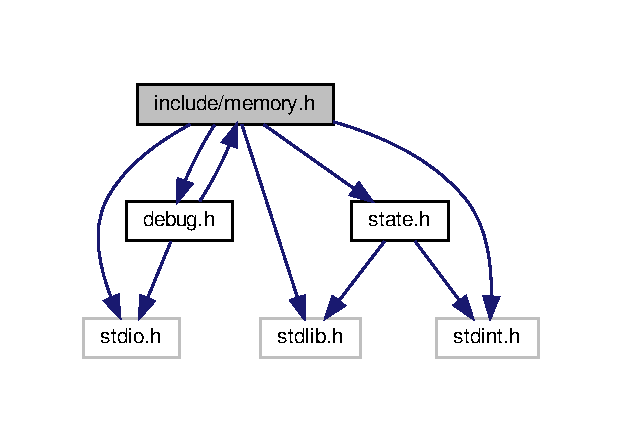
\includegraphics[width=299pt]{memory_8h__incl}
\end{center}
\end{figure}
This graph shows which files directly or indirectly include this file\+:\nopagebreak
\begin{figure}[H]
\begin{center}
\leavevmode
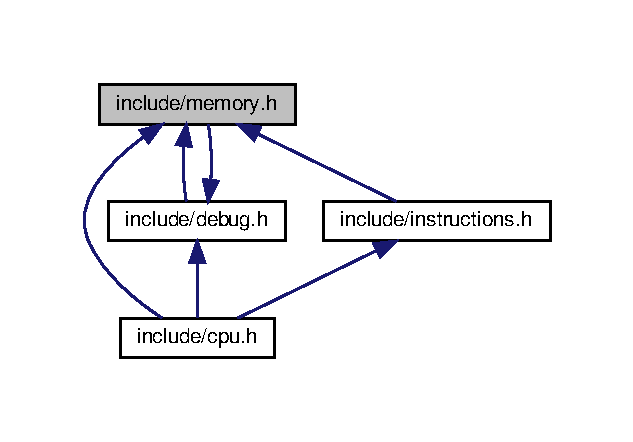
\includegraphics[width=304pt]{memory_8h__dep__incl}
\end{center}
\end{figure}
\subsection*{Macros}
\begin{DoxyCompactItemize}
\item 
\#define \hyperlink{memory_8h_a68419cc4f6bc752ecab770a4da751448}{K\+I\+L\+O\+\_\+\+B\+Y\+TE}~1024
\end{DoxyCompactItemize}
\subsection*{Functions}
\begin{DoxyCompactItemize}
\item 
\mbox{\Hypertarget{memory_8h_ac2cbc1f5e1ab43a1458cdf1bbc79dcb8}\label{memory_8h_ac2cbc1f5e1ab43a1458cdf1bbc79dcb8}} 
void \hyperlink{memory_8h_ac2cbc1f5e1ab43a1458cdf1bbc79dcb8}{Memory\+\_\+init} (void)
\begin{DoxyCompactList}\small\item\em Allocate the emulator\textquotesingle{}s memory and initialize special registers. \end{DoxyCompactList}\item 
\mbox{\Hypertarget{memory_8h_a3991fe5b320be41916cfa3908915fca2}\label{memory_8h_a3991fe5b320be41916cfa3908915fca2}} 
void \hyperlink{memory_8h_a3991fe5b320be41916cfa3908915fca2}{Memory\+\_\+exit} (void)
\begin{DoxyCompactList}\small\item\em Free the allocated memory. \end{DoxyCompactList}\item 
uint8\+\_\+t \hyperlink{memory_8h_a23132297e97c992f33578fd53ecdcfa4}{Memory\+\_\+load\+\_\+byte} (uint16\+\_\+t address)
\begin{DoxyCompactList}\small\item\em Load a byte from the emulator\textquotesingle{}s memory. \end{DoxyCompactList}\item 
void \hyperlink{memory_8h_aee6c781b8a3f54504854cc852314200d}{Memory\+\_\+store\+\_\+byte} (uint16\+\_\+t address, uint8\+\_\+t data)
\begin{DoxyCompactList}\small\item\em Store a byte in the emulator\textquotesingle{}s memory. \end{DoxyCompactList}\item 
uint8\+\_\+t \hyperlink{memory_8h_a25c828bd52fda6442011b6ae3d68a67f}{Memory\+\_\+load\+\_\+byte\+\_\+\+PC} (void)
\begin{DoxyCompactList}\small\item\em Load the byte at the program counter and increment the program counter. \end{DoxyCompactList}\item 
uint16\+\_\+t \hyperlink{memory_8h_a24f868b3fc7b551487bbd9158aaa510d}{Memory\+\_\+load\+\_\+word\+\_\+\+PC} (void)
\begin{DoxyCompactList}\small\item\em Load the 16-\/bit word (L\+SB first) at the program counter and increment the program counter accordingly. \end{DoxyCompactList}\item 
\mbox{\Hypertarget{memory_8h_ac1e824237e4a013ed7d7d5f499292eba}\label{memory_8h_ac1e824237e4a013ed7d7d5f499292eba}} 
void \hyperlink{memory_8h_ac1e824237e4a013ed7d7d5f499292eba}{I\+O\+\_\+init} (void)
\begin{DoxyCompactList}\small\item\em Initialize the special registers in the I\+O-\/section (0x\+F\+F00-\/0x\+F\+F7F) of the memory model. \end{DoxyCompactList}\item 
static void \hyperlink{memory_8h_a781c246713c4f94a67a47f960d25427e}{I\+O\+\_\+store\+\_\+byte} (uint16\+\_\+t address, uint8\+\_\+t data)
\begin{DoxyCompactList}\small\item\em Store a byte in the I\+O-\/section (0x\+F\+F00-\/0x\+F\+F7F) of the memory model. \end{DoxyCompactList}\item 
static uint8\+\_\+t \hyperlink{memory_8h_ad381b9cff8b79f16b07eb82abe485e4a}{I\+O\+\_\+load\+\_\+byte} (uint16\+\_\+t address)
\begin{DoxyCompactList}\small\item\em Load a byte from the I\+O-\/section (0x\+F\+F00-\/0x\+F\+F7F) of the memory model. \end{DoxyCompactList}\end{DoxyCompactItemize}
\subsection*{Variables}
\begin{DoxyCompactItemize}
\item 
\mbox{\Hypertarget{memory_8h_ab6f0ae03120ecb9322e05e1bbc27e364}\label{memory_8h_ab6f0ae03120ecb9322e05e1bbc27e364}} 
\begin{tabbing}
xx\=xx\=xx\=xx\=xx\=xx\=xx\=xx\=xx\=\kill
struct \{\\
\>struct \{\\
\>\>uint8\_t $\ast$ \hyperlink{memory_8h_afa8381d8690dfa1f2bcea5a8e4d00741}{bank\_fixed}\\
\>\>uint8\_t $\ast$ \hyperlink{memory_8h_ac710b75cc62b8885999844bf65b21c78}{bank\_swap}\\
\>\} \hyperlink{memory_8h_a66b23f4199eb5bd14f052087bf83b770}{ROM}\\
\>uint8\_t $\ast$ \hyperlink{memory_8h_abb4726240b8b01131746b0f199c58549}{VRAM}\\
\>uint8\_t $\ast$ \hyperlink{memory_8h_ab1119300a60f06c45d14b0d9eafcf422}{EXTRAM}\\
\>struct \{\\
\>\>uint8\_t $\ast$ \hyperlink{memory_8h_afa8381d8690dfa1f2bcea5a8e4d00741}{bank\_fixed}\\
\>\>uint8\_t $\ast$ \hyperlink{memory_8h_ac710b75cc62b8885999844bf65b21c78}{bank\_swap}\\
\>\} \hyperlink{memory_8h_a792844e460865e8247b08da318142555}{RAM}\\
\>uint8\_t $\ast$ \hyperlink{memory_8h_a199eddb4cf868e571fd2ed01c7a8a32e}{OAM}\\
\>uint8\_t $\ast$ \hyperlink{memory_8h_ac7681f624878a05c3db9eade8b303001}{HRAM}\\
\>uint8\_t \hyperlink{memory_8h_ab1ca70da5c3b3a71451a8b582d9c45ee}{IE}\\
\} \hyperlink{memory_8h_ab6f0ae03120ecb9322e05e1bbc27e364}{Memory}\\

\end{tabbing}\begin{DoxyCompactList}\small\item\em Struct that represents the memory model of the emulator. \end{DoxyCompactList}\item 
\mbox{\Hypertarget{memory_8h_a5f9bd6c1e1c61a55c4dfacc0fb2fa160}\label{memory_8h_a5f9bd6c1e1c61a55c4dfacc0fb2fa160}} 
\begin{tabbing}
xx\=xx\=xx\=xx\=xx\=xx\=xx\=xx\=xx\=\kill
struct \{\\
\>uint8\_t \hyperlink{memory_8h_a89e93cdfda0a253e4d7ba7948fc4d577}{P1}\\
\>uint8\_t \hyperlink{memory_8h_af6e25191020f32790ed358bdb7152678}{SB}\\
\>uint8\_t \hyperlink{memory_8h_a994283cb179a11ded2d18c30c3710802}{SC}\\
\>uint8\_t \hyperlink{memory_8h_aa2c865a3453e463499b654276a70e572}{DIV}\\
\>uint8\_t \hyperlink{memory_8h_ace71b847242f481e21068751bdc85124}{TIMA}\\
\>uint8\_t \hyperlink{memory_8h_ab51e207437a300404935b773224ca546}{TMA}\\
\>uint8\_t \hyperlink{memory_8h_a0c2aed67688f753c0dcaccc4067c472c}{TAC}\\
\>uint8\_t \hyperlink{memory_8h_ae8ee8fbf58d3aeb61d81bae817be8826}{IF}\\
\>uint8\_t \hyperlink{memory_8h_ab1ca70da5c3b3a71451a8b582d9c45ee}{IE}\\
\>uint8\_t \hyperlink{memory_8h_a8fbb8bb9ef49281d646ef1ed0c204a68}{NR10}\\
\>uint8\_t \hyperlink{memory_8h_a01e595f265620d78598813c8653c4f5f}{NR11}\\
\>uint8\_t \hyperlink{memory_8h_ae376586495517abdb6b30bcbf3c594ef}{NR12}\\
\>uint8\_t \hyperlink{memory_8h_a22afb2aa1974dc6c9f1f16c9b189124e}{NR13}\\
\>uint8\_t \hyperlink{memory_8h_a20490b899225cc36d161277515a16e56}{NR14}\\
\>uint8\_t \hyperlink{memory_8h_a030a59f26206ac0ac4201a322b5cdd5d}{NR21}\\
\>uint8\_t \hyperlink{memory_8h_a84a77945673e816e904657cf55b3e902}{NR22}\\
\>uint8\_t \hyperlink{memory_8h_a86f90fa3fd15f1caaee3154f3425ad4f}{NR23}\\
\>uint8\_t \hyperlink{memory_8h_a277721eee408eff8e2bf675da59ab0f2}{NR24}\\
\>uint8\_t \hyperlink{memory_8h_ab1dc91e1df22fd74272e6af40c9f3e22}{NR30}\\
\>uint8\_t \hyperlink{memory_8h_ac27fb79168070f5b8aa58ab030dbc30b}{NR31}\\
\>uint8\_t \hyperlink{memory_8h_a012ca99b3d393d9696a57fbedba071eb}{NR32}\\
\>uint8\_t \hyperlink{memory_8h_ab183837a14028cb6674aaaadd2ac18db}{NR33}\\
\>uint8\_t \hyperlink{memory_8h_aa2b0164adc5f48687ffaf53ac41265b8}{NR34}\\
\>uint8\_t \hyperlink{memory_8h_a5bb89968df1cf6d2724a2b10300fd20f}{NR41}\\
\>uint8\_t \hyperlink{memory_8h_afa29f9e2924c6adb56e8dc67671ff3ac}{NR42}\\
\>uint8\_t \hyperlink{memory_8h_a32e5cc4bcf2df723aeeae24c0c9b3ebe}{NR43}\\
\>uint8\_t \hyperlink{memory_8h_a1012d06d3215a8e5833c8e02146b6c33}{NR44}\\
\>uint8\_t \hyperlink{memory_8h_a01646acd7c6dcf29e7390e9007b6792d}{NR50}\\
\>uint8\_t \hyperlink{memory_8h_ae1d2e83ced05b7401878c591e76def88}{NR51}\\
\>uint8\_t \hyperlink{memory_8h_a0fe259dbbb83d897c6f5e47e04b45a78}{NR52}\\
\>uint8\_t \hyperlink{memory_8h_ada5aa230fbe749561bbcc29c81727bed}{WAVE} \mbox{[}16\mbox{]}\\
\>uint8\_t \hyperlink{memory_8h_a4fef16b094b310f510df6cacf7fa56c6}{LCDC}\\
\>uint8\_t \hyperlink{memory_8h_a29552ccb0992dbc97b7cf8259c0c43fe}{STAT}\\
\>uint8\_t \hyperlink{memory_8h_a9a7b9c16aeab96019096b5d9f509b57f}{SCY}\\
\>uint8\_t \hyperlink{memory_8h_a4ec9bb2eafba7556ff7bd8a2ec8cf1b5}{SCX}\\
\>uint8\_t \hyperlink{memory_8h_aac72867167411ab30a371a9d8e8076d1}{LY}\\
\>uint8\_t \hyperlink{memory_8h_a8ae5a3bf622f470d0e5739b3b427e8a7}{LYC}\\
\>uint8\_t \hyperlink{memory_8h_a6701d95da5fe992e672fbf3925ca2fa4}{DMA}\\
\>uint8\_t \hyperlink{memory_8h_ac547af7ecc2c9b64f2b59c7ad9eed92f}{BGP}\\
\>uint8\_t \hyperlink{memory_8h_a7c04e9a18ac693d6b7ba31764c3ee70e}{OBP0}\\
\>uint8\_t \hyperlink{memory_8h_a53b57174a234f73bc93e80bd543d546a}{OBP1}\\
\>uint8\_t \hyperlink{memory_8h_a623df2e10cad46929fa226da97926eaf}{WY}\\
\>uint8\_t \hyperlink{memory_8h_a26cc5409e89a6f0e14b6da08870fca2d}{WX}\\
\} \hyperlink{memory_8h_a5f9bd6c1e1c61a55c4dfacc0fb2fa160}{IO\_Registers}\\

\end{tabbing}\begin{DoxyCompactList}\small\item\em The hardware registers in the I\+O-\/section of the memory model (0x\+F\+F00-\/0x\+F\+F7F) \end{DoxyCompactList}\end{DoxyCompactItemize}


\subsection{Detailed Description}
Representation of the Game Boy\textquotesingle{}s memory model and operations to read and write to this memory. 

\begin{DoxyAuthor}{Author}
tbnbooij 
\end{DoxyAuthor}
\begin{DoxyDate}{Date}
2018-\/08-\/13 
\end{DoxyDate}


\subsection{Macro Definition Documentation}
\mbox{\Hypertarget{memory_8h_a68419cc4f6bc752ecab770a4da751448}\label{memory_8h_a68419cc4f6bc752ecab770a4da751448}} 
\index{memory.\+h@{memory.\+h}!K\+I\+L\+O\+\_\+\+B\+Y\+TE@{K\+I\+L\+O\+\_\+\+B\+Y\+TE}}
\index{K\+I\+L\+O\+\_\+\+B\+Y\+TE@{K\+I\+L\+O\+\_\+\+B\+Y\+TE}!memory.\+h@{memory.\+h}}
\subsubsection{\texorpdfstring{K\+I\+L\+O\+\_\+\+B\+Y\+TE}{KILO\_BYTE}}
{\footnotesize\ttfamily \#define K\+I\+L\+O\+\_\+\+B\+Y\+TE~1024}

Size of a kilobyte in bytes 

\subsection{Function Documentation}
\mbox{\Hypertarget{memory_8h_ad381b9cff8b79f16b07eb82abe485e4a}\label{memory_8h_ad381b9cff8b79f16b07eb82abe485e4a}} 
\index{memory.\+h@{memory.\+h}!I\+O\+\_\+load\+\_\+byte@{I\+O\+\_\+load\+\_\+byte}}
\index{I\+O\+\_\+load\+\_\+byte@{I\+O\+\_\+load\+\_\+byte}!memory.\+h@{memory.\+h}}
\subsubsection{\texorpdfstring{I\+O\+\_\+load\+\_\+byte()}{IO\_load\_byte()}}
{\footnotesize\ttfamily static uint8\+\_\+t I\+O\+\_\+load\+\_\+byte (\begin{DoxyParamCaption}\item[{uint16\+\_\+t}]{address }\end{DoxyParamCaption})\hspace{0.3cm}{\ttfamily [static]}}



Load a byte from the I\+O-\/section (0x\+F\+F00-\/0x\+F\+F7F) of the memory model. 


\begin{DoxyParams}{Parameters}
{\em address} & The address of a byte in the I\+O-\/section \\
\hline
\end{DoxyParams}
\begin{DoxyReturn}{Returns}
uint8\+\_\+t The value at the given address 
\end{DoxyReturn}
\mbox{\Hypertarget{memory_8h_a781c246713c4f94a67a47f960d25427e}\label{memory_8h_a781c246713c4f94a67a47f960d25427e}} 
\index{memory.\+h@{memory.\+h}!I\+O\+\_\+store\+\_\+byte@{I\+O\+\_\+store\+\_\+byte}}
\index{I\+O\+\_\+store\+\_\+byte@{I\+O\+\_\+store\+\_\+byte}!memory.\+h@{memory.\+h}}
\subsubsection{\texorpdfstring{I\+O\+\_\+store\+\_\+byte()}{IO\_store\_byte()}}
{\footnotesize\ttfamily static void I\+O\+\_\+store\+\_\+byte (\begin{DoxyParamCaption}\item[{uint16\+\_\+t}]{address,  }\item[{uint8\+\_\+t}]{data }\end{DoxyParamCaption})\hspace{0.3cm}{\ttfamily [static]}}



Store a byte in the I\+O-\/section (0x\+F\+F00-\/0x\+F\+F7F) of the memory model. 


\begin{DoxyParams}{Parameters}
{\em address} & The address of a byte in the I\+O-\/section \\
\hline
{\em data} & The value to be stored \\
\hline
\end{DoxyParams}
\mbox{\Hypertarget{memory_8h_a23132297e97c992f33578fd53ecdcfa4}\label{memory_8h_a23132297e97c992f33578fd53ecdcfa4}} 
\index{memory.\+h@{memory.\+h}!Memory\+\_\+load\+\_\+byte@{Memory\+\_\+load\+\_\+byte}}
\index{Memory\+\_\+load\+\_\+byte@{Memory\+\_\+load\+\_\+byte}!memory.\+h@{memory.\+h}}
\subsubsection{\texorpdfstring{Memory\+\_\+load\+\_\+byte()}{Memory\_load\_byte()}}
{\footnotesize\ttfamily uint8\+\_\+t Memory\+\_\+load\+\_\+byte (\begin{DoxyParamCaption}\item[{uint16\+\_\+t}]{address }\end{DoxyParamCaption})}



Load a byte from the emulator\textquotesingle{}s memory. 


\begin{DoxyParams}{Parameters}
{\em address} & The 16-\/bit address of the read byte \\
\hline
\end{DoxyParams}
\begin{DoxyReturn}{Returns}
uint8\+\_\+t The value at the given address 
\end{DoxyReturn}
\mbox{\Hypertarget{memory_8h_a25c828bd52fda6442011b6ae3d68a67f}\label{memory_8h_a25c828bd52fda6442011b6ae3d68a67f}} 
\index{memory.\+h@{memory.\+h}!Memory\+\_\+load\+\_\+byte\+\_\+\+PC@{Memory\+\_\+load\+\_\+byte\+\_\+\+PC}}
\index{Memory\+\_\+load\+\_\+byte\+\_\+\+PC@{Memory\+\_\+load\+\_\+byte\+\_\+\+PC}!memory.\+h@{memory.\+h}}
\subsubsection{\texorpdfstring{Memory\+\_\+load\+\_\+byte\+\_\+\+P\+C()}{Memory\_load\_byte\_PC()}}
{\footnotesize\ttfamily uint8\+\_\+t Memory\+\_\+load\+\_\+byte\+\_\+\+PC (\begin{DoxyParamCaption}\item[{void}]{ }\end{DoxyParamCaption})}



Load the byte at the program counter and increment the program counter. 

\begin{DoxyReturn}{Returns}
uint8\+\_\+t The value at the program counter 
\end{DoxyReturn}
\mbox{\Hypertarget{memory_8h_a24f868b3fc7b551487bbd9158aaa510d}\label{memory_8h_a24f868b3fc7b551487bbd9158aaa510d}} 
\index{memory.\+h@{memory.\+h}!Memory\+\_\+load\+\_\+word\+\_\+\+PC@{Memory\+\_\+load\+\_\+word\+\_\+\+PC}}
\index{Memory\+\_\+load\+\_\+word\+\_\+\+PC@{Memory\+\_\+load\+\_\+word\+\_\+\+PC}!memory.\+h@{memory.\+h}}
\subsubsection{\texorpdfstring{Memory\+\_\+load\+\_\+word\+\_\+\+P\+C()}{Memory\_load\_word\_PC()}}
{\footnotesize\ttfamily uint16\+\_\+t Memory\+\_\+load\+\_\+word\+\_\+\+PC (\begin{DoxyParamCaption}\item[{void}]{ }\end{DoxyParamCaption})}



Load the 16-\/bit word (L\+SB first) at the program counter and increment the program counter accordingly. 

\begin{DoxyReturn}{Returns}
uint16\+\_\+t The 16-\/bit value read at the program counter 
\end{DoxyReturn}
\mbox{\Hypertarget{memory_8h_aee6c781b8a3f54504854cc852314200d}\label{memory_8h_aee6c781b8a3f54504854cc852314200d}} 
\index{memory.\+h@{memory.\+h}!Memory\+\_\+store\+\_\+byte@{Memory\+\_\+store\+\_\+byte}}
\index{Memory\+\_\+store\+\_\+byte@{Memory\+\_\+store\+\_\+byte}!memory.\+h@{memory.\+h}}
\subsubsection{\texorpdfstring{Memory\+\_\+store\+\_\+byte()}{Memory\_store\_byte()}}
{\footnotesize\ttfamily void Memory\+\_\+store\+\_\+byte (\begin{DoxyParamCaption}\item[{uint16\+\_\+t}]{address,  }\item[{uint8\+\_\+t}]{data }\end{DoxyParamCaption})}



Store a byte in the emulator\textquotesingle{}s memory. 


\begin{DoxyParams}{Parameters}
{\em address} & The 16-\/bit address where the byte will be stored \\
\hline
{\em data} & The value that will be stored \\
\hline
\end{DoxyParams}


\subsection{Variable Documentation}
\mbox{\Hypertarget{memory_8h_afa8381d8690dfa1f2bcea5a8e4d00741}\label{memory_8h_afa8381d8690dfa1f2bcea5a8e4d00741}} 
\index{memory.\+h@{memory.\+h}!bank\+\_\+fixed@{bank\+\_\+fixed}}
\index{bank\+\_\+fixed@{bank\+\_\+fixed}!memory.\+h@{memory.\+h}}
\subsubsection{\texorpdfstring{bank\+\_\+fixed}{bank\_fixed}}
{\footnotesize\ttfamily uint8\+\_\+t$\ast$ bank\+\_\+fixed}

8 kB block of R\+OM that cannot be swapped by a memory bank controller (0x0000-\/0x3\+F\+FF)

4 kB of internal R\+AM that cannot be swapped by an internal memory bank controller (0x\+C000-\/0x\+C\+F\+FF) \mbox{\Hypertarget{memory_8h_ac710b75cc62b8885999844bf65b21c78}\label{memory_8h_ac710b75cc62b8885999844bf65b21c78}} 
\index{memory.\+h@{memory.\+h}!bank\+\_\+swap@{bank\+\_\+swap}}
\index{bank\+\_\+swap@{bank\+\_\+swap}!memory.\+h@{memory.\+h}}
\subsubsection{\texorpdfstring{bank\+\_\+swap}{bank\_swap}}
{\footnotesize\ttfamily uint8\+\_\+t$\ast$ bank\+\_\+swap}

8 kB block of R\+OM that may be swapped by the memory bank controller (0x4000-\/0x7\+F\+FF)

4 kB of internal R\+AM that may be swapped by an internal memory bank controller (C\+GB only; 0x\+D000-\/0x\+D\+F\+FF) \mbox{\Hypertarget{memory_8h_ac547af7ecc2c9b64f2b59c7ad9eed92f}\label{memory_8h_ac547af7ecc2c9b64f2b59c7ad9eed92f}} 
\index{memory.\+h@{memory.\+h}!B\+GP@{B\+GP}}
\index{B\+GP@{B\+GP}!memory.\+h@{memory.\+h}}
\subsubsection{\texorpdfstring{B\+GP}{BGP}}
{\footnotesize\ttfamily uint8\+\_\+t B\+GP}

(0x\+F\+F47) Background and window palette data (R/W) \mbox{\Hypertarget{memory_8h_aa2c865a3453e463499b654276a70e572}\label{memory_8h_aa2c865a3453e463499b654276a70e572}} 
\index{memory.\+h@{memory.\+h}!D\+IV@{D\+IV}}
\index{D\+IV@{D\+IV}!memory.\+h@{memory.\+h}}
\subsubsection{\texorpdfstring{D\+IV}{DIV}}
{\footnotesize\ttfamily uint8\+\_\+t D\+IV}

(0x\+F\+F03) Divider register (R/W) \mbox{\Hypertarget{memory_8h_a6701d95da5fe992e672fbf3925ca2fa4}\label{memory_8h_a6701d95da5fe992e672fbf3925ca2fa4}} 
\index{memory.\+h@{memory.\+h}!D\+MA@{D\+MA}}
\index{D\+MA@{D\+MA}!memory.\+h@{memory.\+h}}
\subsubsection{\texorpdfstring{D\+MA}{DMA}}
{\footnotesize\ttfamily uint8\+\_\+t D\+MA}

(0x\+F\+F46) D\+MA transfer and start address (W) \mbox{\Hypertarget{memory_8h_ab1119300a60f06c45d14b0d9eafcf422}\label{memory_8h_ab1119300a60f06c45d14b0d9eafcf422}} 
\index{memory.\+h@{memory.\+h}!E\+X\+T\+R\+AM@{E\+X\+T\+R\+AM}}
\index{E\+X\+T\+R\+AM@{E\+X\+T\+R\+AM}!memory.\+h@{memory.\+h}}
\subsubsection{\texorpdfstring{E\+X\+T\+R\+AM}{EXTRAM}}
{\footnotesize\ttfamily uint8\+\_\+t$\ast$ E\+X\+T\+R\+AM}

External R\+AM that may or may not be provided by a game cartridge (0x\+A000-\/0x\+B\+F\+FF) \mbox{\Hypertarget{memory_8h_ac7681f624878a05c3db9eade8b303001}\label{memory_8h_ac7681f624878a05c3db9eade8b303001}} 
\index{memory.\+h@{memory.\+h}!H\+R\+AM@{H\+R\+AM}}
\index{H\+R\+AM@{H\+R\+AM}!memory.\+h@{memory.\+h}}
\subsubsection{\texorpdfstring{H\+R\+AM}{HRAM}}
{\footnotesize\ttfamily uint8\+\_\+t$\ast$ H\+R\+AM}

High R\+A\+M/\+Zero page (0x\+F\+F80-\/0x\+F\+F\+FE) \mbox{\Hypertarget{memory_8h_ab1ca70da5c3b3a71451a8b582d9c45ee}\label{memory_8h_ab1ca70da5c3b3a71451a8b582d9c45ee}} 
\index{memory.\+h@{memory.\+h}!IE@{IE}}
\index{IE@{IE}!memory.\+h@{memory.\+h}}
\subsubsection{\texorpdfstring{IE}{IE}}
{\footnotesize\ttfamily uint8\+\_\+t IE}

Interrupt enable flag (0x\+F\+F\+FF)

(0x\+F\+F\+FF) Interrupt enable flag (R/W) \mbox{\Hypertarget{memory_8h_ae8ee8fbf58d3aeb61d81bae817be8826}\label{memory_8h_ae8ee8fbf58d3aeb61d81bae817be8826}} 
\index{memory.\+h@{memory.\+h}!IF@{IF}}
\index{IF@{IF}!memory.\+h@{memory.\+h}}
\subsubsection{\texorpdfstring{IF}{IF}}
{\footnotesize\ttfamily uint8\+\_\+t IF}

(0x\+F\+F0F) Interrupt flag (R/W) \mbox{\Hypertarget{memory_8h_a4fef16b094b310f510df6cacf7fa56c6}\label{memory_8h_a4fef16b094b310f510df6cacf7fa56c6}} 
\index{memory.\+h@{memory.\+h}!L\+C\+DC@{L\+C\+DC}}
\index{L\+C\+DC@{L\+C\+DC}!memory.\+h@{memory.\+h}}
\subsubsection{\texorpdfstring{L\+C\+DC}{LCDC}}
{\footnotesize\ttfamily uint8\+\_\+t L\+C\+DC}

(0x\+F\+F40) L\+CD control (R/W) \mbox{\Hypertarget{memory_8h_aac72867167411ab30a371a9d8e8076d1}\label{memory_8h_aac72867167411ab30a371a9d8e8076d1}} 
\index{memory.\+h@{memory.\+h}!LY@{LY}}
\index{LY@{LY}!memory.\+h@{memory.\+h}}
\subsubsection{\texorpdfstring{LY}{LY}}
{\footnotesize\ttfamily uint8\+\_\+t LY}

(0x\+F\+F44) L\+C\+DC Y-\/coordinate (R/W) \mbox{\Hypertarget{memory_8h_a8ae5a3bf622f470d0e5739b3b427e8a7}\label{memory_8h_a8ae5a3bf622f470d0e5739b3b427e8a7}} 
\index{memory.\+h@{memory.\+h}!L\+YC@{L\+YC}}
\index{L\+YC@{L\+YC}!memory.\+h@{memory.\+h}}
\subsubsection{\texorpdfstring{L\+YC}{LYC}}
{\footnotesize\ttfamily uint8\+\_\+t L\+YC}

(0x\+F\+F45) LY compare (R/W) \mbox{\Hypertarget{memory_8h_a8fbb8bb9ef49281d646ef1ed0c204a68}\label{memory_8h_a8fbb8bb9ef49281d646ef1ed0c204a68}} 
\index{memory.\+h@{memory.\+h}!N\+R10@{N\+R10}}
\index{N\+R10@{N\+R10}!memory.\+h@{memory.\+h}}
\subsubsection{\texorpdfstring{N\+R10}{NR10}}
{\footnotesize\ttfamily uint8\+\_\+t N\+R10}

(0x\+F\+F10) Sound mode 1 register; sweep register (R/W) \mbox{\Hypertarget{memory_8h_a01e595f265620d78598813c8653c4f5f}\label{memory_8h_a01e595f265620d78598813c8653c4f5f}} 
\index{memory.\+h@{memory.\+h}!N\+R11@{N\+R11}}
\index{N\+R11@{N\+R11}!memory.\+h@{memory.\+h}}
\subsubsection{\texorpdfstring{N\+R11}{NR11}}
{\footnotesize\ttfamily uint8\+\_\+t N\+R11}

(0x\+F\+F11) Sound mode 1 register; sound length/wave pattern duty (R/W) \mbox{\Hypertarget{memory_8h_ae376586495517abdb6b30bcbf3c594ef}\label{memory_8h_ae376586495517abdb6b30bcbf3c594ef}} 
\index{memory.\+h@{memory.\+h}!N\+R12@{N\+R12}}
\index{N\+R12@{N\+R12}!memory.\+h@{memory.\+h}}
\subsubsection{\texorpdfstring{N\+R12}{NR12}}
{\footnotesize\ttfamily uint8\+\_\+t N\+R12}

(0x\+F\+F12) Sound mode 1 register; envelope (R/W) \mbox{\Hypertarget{memory_8h_a22afb2aa1974dc6c9f1f16c9b189124e}\label{memory_8h_a22afb2aa1974dc6c9f1f16c9b189124e}} 
\index{memory.\+h@{memory.\+h}!N\+R13@{N\+R13}}
\index{N\+R13@{N\+R13}!memory.\+h@{memory.\+h}}
\subsubsection{\texorpdfstring{N\+R13}{NR13}}
{\footnotesize\ttfamily uint8\+\_\+t N\+R13}

(0x\+F\+F13) Sound mode 1 register; frequency lo (W) \mbox{\Hypertarget{memory_8h_a20490b899225cc36d161277515a16e56}\label{memory_8h_a20490b899225cc36d161277515a16e56}} 
\index{memory.\+h@{memory.\+h}!N\+R14@{N\+R14}}
\index{N\+R14@{N\+R14}!memory.\+h@{memory.\+h}}
\subsubsection{\texorpdfstring{N\+R14}{NR14}}
{\footnotesize\ttfamily uint8\+\_\+t N\+R14}

(0x\+F\+F14) Sound mode 1 register; frequency hi (W) \mbox{\Hypertarget{memory_8h_a030a59f26206ac0ac4201a322b5cdd5d}\label{memory_8h_a030a59f26206ac0ac4201a322b5cdd5d}} 
\index{memory.\+h@{memory.\+h}!N\+R21@{N\+R21}}
\index{N\+R21@{N\+R21}!memory.\+h@{memory.\+h}}
\subsubsection{\texorpdfstring{N\+R21}{NR21}}
{\footnotesize\ttfamily uint8\+\_\+t N\+R21}

(0x\+F\+F16) Sound mode 2 register; sound length/wave pattern duty (R/W) \mbox{\Hypertarget{memory_8h_a84a77945673e816e904657cf55b3e902}\label{memory_8h_a84a77945673e816e904657cf55b3e902}} 
\index{memory.\+h@{memory.\+h}!N\+R22@{N\+R22}}
\index{N\+R22@{N\+R22}!memory.\+h@{memory.\+h}}
\subsubsection{\texorpdfstring{N\+R22}{NR22}}
{\footnotesize\ttfamily uint8\+\_\+t N\+R22}

(0x\+F\+F17) Sound mode 2 register; envelope (R/W) \mbox{\Hypertarget{memory_8h_a86f90fa3fd15f1caaee3154f3425ad4f}\label{memory_8h_a86f90fa3fd15f1caaee3154f3425ad4f}} 
\index{memory.\+h@{memory.\+h}!N\+R23@{N\+R23}}
\index{N\+R23@{N\+R23}!memory.\+h@{memory.\+h}}
\subsubsection{\texorpdfstring{N\+R23}{NR23}}
{\footnotesize\ttfamily uint8\+\_\+t N\+R23}

(0x\+F\+F18) Sound mode 2 register; frequency lo (W) \mbox{\Hypertarget{memory_8h_a277721eee408eff8e2bf675da59ab0f2}\label{memory_8h_a277721eee408eff8e2bf675da59ab0f2}} 
\index{memory.\+h@{memory.\+h}!N\+R24@{N\+R24}}
\index{N\+R24@{N\+R24}!memory.\+h@{memory.\+h}}
\subsubsection{\texorpdfstring{N\+R24}{NR24}}
{\footnotesize\ttfamily uint8\+\_\+t N\+R24}

(0x\+F\+F19) Sound mode 2 register; frequency hi (R/W) \mbox{\Hypertarget{memory_8h_ab1dc91e1df22fd74272e6af40c9f3e22}\label{memory_8h_ab1dc91e1df22fd74272e6af40c9f3e22}} 
\index{memory.\+h@{memory.\+h}!N\+R30@{N\+R30}}
\index{N\+R30@{N\+R30}!memory.\+h@{memory.\+h}}
\subsubsection{\texorpdfstring{N\+R30}{NR30}}
{\footnotesize\ttfamily uint8\+\_\+t N\+R30}

(0x\+F\+F1A) Sound mode 3 register; sound on/off (R/W) \mbox{\Hypertarget{memory_8h_ac27fb79168070f5b8aa58ab030dbc30b}\label{memory_8h_ac27fb79168070f5b8aa58ab030dbc30b}} 
\index{memory.\+h@{memory.\+h}!N\+R31@{N\+R31}}
\index{N\+R31@{N\+R31}!memory.\+h@{memory.\+h}}
\subsubsection{\texorpdfstring{N\+R31}{NR31}}
{\footnotesize\ttfamily uint8\+\_\+t N\+R31}

(0x\+F\+F1B) Sound mode 3 register; sound length (R/W) \mbox{\Hypertarget{memory_8h_a012ca99b3d393d9696a57fbedba071eb}\label{memory_8h_a012ca99b3d393d9696a57fbedba071eb}} 
\index{memory.\+h@{memory.\+h}!N\+R32@{N\+R32}}
\index{N\+R32@{N\+R32}!memory.\+h@{memory.\+h}}
\subsubsection{\texorpdfstring{N\+R32}{NR32}}
{\footnotesize\ttfamily uint8\+\_\+t N\+R32}

(0x\+F\+F1C) Sound mode 3 register, select output level (R/W) \mbox{\Hypertarget{memory_8h_ab183837a14028cb6674aaaadd2ac18db}\label{memory_8h_ab183837a14028cb6674aaaadd2ac18db}} 
\index{memory.\+h@{memory.\+h}!N\+R33@{N\+R33}}
\index{N\+R33@{N\+R33}!memory.\+h@{memory.\+h}}
\subsubsection{\texorpdfstring{N\+R33}{NR33}}
{\footnotesize\ttfamily uint8\+\_\+t N\+R33}

(0x\+F\+F1D) Sound mode 3 register; frequency lo (W) \mbox{\Hypertarget{memory_8h_aa2b0164adc5f48687ffaf53ac41265b8}\label{memory_8h_aa2b0164adc5f48687ffaf53ac41265b8}} 
\index{memory.\+h@{memory.\+h}!N\+R34@{N\+R34}}
\index{N\+R34@{N\+R34}!memory.\+h@{memory.\+h}}
\subsubsection{\texorpdfstring{N\+R34}{NR34}}
{\footnotesize\ttfamily uint8\+\_\+t N\+R34}

(0x\+F\+F1E) Sound mode 3 register; frequency hi (R/W) \mbox{\Hypertarget{memory_8h_a5bb89968df1cf6d2724a2b10300fd20f}\label{memory_8h_a5bb89968df1cf6d2724a2b10300fd20f}} 
\index{memory.\+h@{memory.\+h}!N\+R41@{N\+R41}}
\index{N\+R41@{N\+R41}!memory.\+h@{memory.\+h}}
\subsubsection{\texorpdfstring{N\+R41}{NR41}}
{\footnotesize\ttfamily uint8\+\_\+t N\+R41}

(0x\+F\+F20) Sound mode 4 register; sound length (R/W) \mbox{\Hypertarget{memory_8h_afa29f9e2924c6adb56e8dc67671ff3ac}\label{memory_8h_afa29f9e2924c6adb56e8dc67671ff3ac}} 
\index{memory.\+h@{memory.\+h}!N\+R42@{N\+R42}}
\index{N\+R42@{N\+R42}!memory.\+h@{memory.\+h}}
\subsubsection{\texorpdfstring{N\+R42}{NR42}}
{\footnotesize\ttfamily uint8\+\_\+t N\+R42}

(0x\+F\+F21) Sound mode 4 register; envelope (R/W) \mbox{\Hypertarget{memory_8h_a32e5cc4bcf2df723aeeae24c0c9b3ebe}\label{memory_8h_a32e5cc4bcf2df723aeeae24c0c9b3ebe}} 
\index{memory.\+h@{memory.\+h}!N\+R43@{N\+R43}}
\index{N\+R43@{N\+R43}!memory.\+h@{memory.\+h}}
\subsubsection{\texorpdfstring{N\+R43}{NR43}}
{\footnotesize\ttfamily uint8\+\_\+t N\+R43}

(0x\+F\+F22) Sound mode 4 register; polynomial counter (R/W) \mbox{\Hypertarget{memory_8h_a1012d06d3215a8e5833c8e02146b6c33}\label{memory_8h_a1012d06d3215a8e5833c8e02146b6c33}} 
\index{memory.\+h@{memory.\+h}!N\+R44@{N\+R44}}
\index{N\+R44@{N\+R44}!memory.\+h@{memory.\+h}}
\subsubsection{\texorpdfstring{N\+R44}{NR44}}
{\footnotesize\ttfamily uint8\+\_\+t N\+R44}

(0x\+F\+F23) Sound mode 4 register; counter/consecutive; initial (R/W) \mbox{\Hypertarget{memory_8h_a01646acd7c6dcf29e7390e9007b6792d}\label{memory_8h_a01646acd7c6dcf29e7390e9007b6792d}} 
\index{memory.\+h@{memory.\+h}!N\+R50@{N\+R50}}
\index{N\+R50@{N\+R50}!memory.\+h@{memory.\+h}}
\subsubsection{\texorpdfstring{N\+R50}{NR50}}
{\footnotesize\ttfamily uint8\+\_\+t N\+R50}

(0x\+F\+F24) Channel control / O\+N-\/\+O\+FF / volume (R/W) \mbox{\Hypertarget{memory_8h_ae1d2e83ced05b7401878c591e76def88}\label{memory_8h_ae1d2e83ced05b7401878c591e76def88}} 
\index{memory.\+h@{memory.\+h}!N\+R51@{N\+R51}}
\index{N\+R51@{N\+R51}!memory.\+h@{memory.\+h}}
\subsubsection{\texorpdfstring{N\+R51}{NR51}}
{\footnotesize\ttfamily uint8\+\_\+t N\+R51}

(0x\+F\+F25) Selection of sound output terminal (R/W) \mbox{\Hypertarget{memory_8h_a0fe259dbbb83d897c6f5e47e04b45a78}\label{memory_8h_a0fe259dbbb83d897c6f5e47e04b45a78}} 
\index{memory.\+h@{memory.\+h}!N\+R52@{N\+R52}}
\index{N\+R52@{N\+R52}!memory.\+h@{memory.\+h}}
\subsubsection{\texorpdfstring{N\+R52}{NR52}}
{\footnotesize\ttfamily uint8\+\_\+t N\+R52}

(0x\+F\+F26) Sound on/off (R/W) \mbox{\Hypertarget{memory_8h_a199eddb4cf868e571fd2ed01c7a8a32e}\label{memory_8h_a199eddb4cf868e571fd2ed01c7a8a32e}} 
\index{memory.\+h@{memory.\+h}!O\+AM@{O\+AM}}
\index{O\+AM@{O\+AM}!memory.\+h@{memory.\+h}}
\subsubsection{\texorpdfstring{O\+AM}{OAM}}
{\footnotesize\ttfamily uint8\+\_\+t$\ast$ O\+AM}

Object Attribute Memory, stores the state of the sprites (0x\+F\+E00-\/0x\+F\+E9F) \mbox{\Hypertarget{memory_8h_a7c04e9a18ac693d6b7ba31764c3ee70e}\label{memory_8h_a7c04e9a18ac693d6b7ba31764c3ee70e}} 
\index{memory.\+h@{memory.\+h}!O\+B\+P0@{O\+B\+P0}}
\index{O\+B\+P0@{O\+B\+P0}!memory.\+h@{memory.\+h}}
\subsubsection{\texorpdfstring{O\+B\+P0}{OBP0}}
{\footnotesize\ttfamily uint8\+\_\+t O\+B\+P0}

(0x\+F\+F48) Object palette 0 data (R/W) \mbox{\Hypertarget{memory_8h_a53b57174a234f73bc93e80bd543d546a}\label{memory_8h_a53b57174a234f73bc93e80bd543d546a}} 
\index{memory.\+h@{memory.\+h}!O\+B\+P1@{O\+B\+P1}}
\index{O\+B\+P1@{O\+B\+P1}!memory.\+h@{memory.\+h}}
\subsubsection{\texorpdfstring{O\+B\+P1}{OBP1}}
{\footnotesize\ttfamily uint8\+\_\+t O\+B\+P1}

(0x\+F\+F49) Object palette 1 data (R/W) \mbox{\Hypertarget{memory_8h_a89e93cdfda0a253e4d7ba7948fc4d577}\label{memory_8h_a89e93cdfda0a253e4d7ba7948fc4d577}} 
\index{memory.\+h@{memory.\+h}!P1@{P1}}
\index{P1@{P1}!memory.\+h@{memory.\+h}}
\subsubsection{\texorpdfstring{P1}{P1}}
{\footnotesize\ttfamily uint8\+\_\+t P1}

(0x\+F\+F00) Register for reading joy pad info and determining system type (R/W) \mbox{\Hypertarget{memory_8h_a792844e460865e8247b08da318142555}\label{memory_8h_a792844e460865e8247b08da318142555}} 
\index{memory.\+h@{memory.\+h}!R\+AM@{R\+AM}}
\index{R\+AM@{R\+AM}!memory.\+h@{memory.\+h}}
\subsubsection{\texorpdfstring{R\+AM}{RAM}}
{\footnotesize\ttfamily struct \{ ... \}   R\+AM}

Internal R\+AM of the Game Boy (0x\+C000-\/0x\+D\+F\+FF) \mbox{\Hypertarget{memory_8h_a66b23f4199eb5bd14f052087bf83b770}\label{memory_8h_a66b23f4199eb5bd14f052087bf83b770}} 
\index{memory.\+h@{memory.\+h}!R\+OM@{R\+OM}}
\index{R\+OM@{R\+OM}!memory.\+h@{memory.\+h}}
\subsubsection{\texorpdfstring{R\+OM}{ROM}}
{\footnotesize\ttfamily struct \{ ... \}   R\+OM}

The read-\/only memory as stored in the game cartrige and (potentially) controlled by a memory bank controller \mbox{\Hypertarget{memory_8h_af6e25191020f32790ed358bdb7152678}\label{memory_8h_af6e25191020f32790ed358bdb7152678}} 
\index{memory.\+h@{memory.\+h}!SB@{SB}}
\index{SB@{SB}!memory.\+h@{memory.\+h}}
\subsubsection{\texorpdfstring{SB}{SB}}
{\footnotesize\ttfamily uint8\+\_\+t SB}

(0x\+F\+F01) Serial transfer data (R/W) \mbox{\Hypertarget{memory_8h_a994283cb179a11ded2d18c30c3710802}\label{memory_8h_a994283cb179a11ded2d18c30c3710802}} 
\index{memory.\+h@{memory.\+h}!SC@{SC}}
\index{SC@{SC}!memory.\+h@{memory.\+h}}
\subsubsection{\texorpdfstring{SC}{SC}}
{\footnotesize\ttfamily uint8\+\_\+t SC}

(0x\+F\+F02) S\+IO control (R/W) \mbox{\Hypertarget{memory_8h_a4ec9bb2eafba7556ff7bd8a2ec8cf1b5}\label{memory_8h_a4ec9bb2eafba7556ff7bd8a2ec8cf1b5}} 
\index{memory.\+h@{memory.\+h}!S\+CX@{S\+CX}}
\index{S\+CX@{S\+CX}!memory.\+h@{memory.\+h}}
\subsubsection{\texorpdfstring{S\+CX}{SCX}}
{\footnotesize\ttfamily uint8\+\_\+t S\+CX}

(0x\+F\+F43) Scroll X (R/W) \mbox{\Hypertarget{memory_8h_a9a7b9c16aeab96019096b5d9f509b57f}\label{memory_8h_a9a7b9c16aeab96019096b5d9f509b57f}} 
\index{memory.\+h@{memory.\+h}!S\+CY@{S\+CY}}
\index{S\+CY@{S\+CY}!memory.\+h@{memory.\+h}}
\subsubsection{\texorpdfstring{S\+CY}{SCY}}
{\footnotesize\ttfamily uint8\+\_\+t S\+CY}

(0x\+F\+F42) Scroll Y (R/W) \mbox{\Hypertarget{memory_8h_a29552ccb0992dbc97b7cf8259c0c43fe}\label{memory_8h_a29552ccb0992dbc97b7cf8259c0c43fe}} 
\index{memory.\+h@{memory.\+h}!S\+T\+AT@{S\+T\+AT}}
\index{S\+T\+AT@{S\+T\+AT}!memory.\+h@{memory.\+h}}
\subsubsection{\texorpdfstring{S\+T\+AT}{STAT}}
{\footnotesize\ttfamily uint8\+\_\+t S\+T\+AT}

(0x\+F\+F41) L\+C\+DC status (R/W) \mbox{\Hypertarget{memory_8h_a0c2aed67688f753c0dcaccc4067c472c}\label{memory_8h_a0c2aed67688f753c0dcaccc4067c472c}} 
\index{memory.\+h@{memory.\+h}!T\+AC@{T\+AC}}
\index{T\+AC@{T\+AC}!memory.\+h@{memory.\+h}}
\subsubsection{\texorpdfstring{T\+AC}{TAC}}
{\footnotesize\ttfamily uint8\+\_\+t T\+AC}

(0x\+F\+F07) Timer control (R/W) \mbox{\Hypertarget{memory_8h_ace71b847242f481e21068751bdc85124}\label{memory_8h_ace71b847242f481e21068751bdc85124}} 
\index{memory.\+h@{memory.\+h}!T\+I\+MA@{T\+I\+MA}}
\index{T\+I\+MA@{T\+I\+MA}!memory.\+h@{memory.\+h}}
\subsubsection{\texorpdfstring{T\+I\+MA}{TIMA}}
{\footnotesize\ttfamily uint8\+\_\+t T\+I\+MA}

(0x\+F\+F05) Timer counter (R/W) \mbox{\Hypertarget{memory_8h_ab51e207437a300404935b773224ca546}\label{memory_8h_ab51e207437a300404935b773224ca546}} 
\index{memory.\+h@{memory.\+h}!T\+MA@{T\+MA}}
\index{T\+MA@{T\+MA}!memory.\+h@{memory.\+h}}
\subsubsection{\texorpdfstring{T\+MA}{TMA}}
{\footnotesize\ttfamily uint8\+\_\+t T\+MA}

(0x\+F\+F06) Timer modulo (R/W) \mbox{\Hypertarget{memory_8h_abb4726240b8b01131746b0f199c58549}\label{memory_8h_abb4726240b8b01131746b0f199c58549}} 
\index{memory.\+h@{memory.\+h}!V\+R\+AM@{V\+R\+AM}}
\index{V\+R\+AM@{V\+R\+AM}!memory.\+h@{memory.\+h}}
\subsubsection{\texorpdfstring{V\+R\+AM}{VRAM}}
{\footnotesize\ttfamily uint8\+\_\+t$\ast$ V\+R\+AM}

The video R\+AM of the Game Boy (0x8000-\/0x9\+F\+FF) \mbox{\Hypertarget{memory_8h_ada5aa230fbe749561bbcc29c81727bed}\label{memory_8h_ada5aa230fbe749561bbcc29c81727bed}} 
\index{memory.\+h@{memory.\+h}!W\+A\+VE@{W\+A\+VE}}
\index{W\+A\+VE@{W\+A\+VE}!memory.\+h@{memory.\+h}}
\subsubsection{\texorpdfstring{W\+A\+VE}{WAVE}}
{\footnotesize\ttfamily uint8\+\_\+t W\+A\+VE\mbox{[}16\mbox{]}}

(0x\+F\+F30-\/0x\+F\+F3F) Waveform storage for arbitrary sound data \mbox{\Hypertarget{memory_8h_a26cc5409e89a6f0e14b6da08870fca2d}\label{memory_8h_a26cc5409e89a6f0e14b6da08870fca2d}} 
\index{memory.\+h@{memory.\+h}!WX@{WX}}
\index{WX@{WX}!memory.\+h@{memory.\+h}}
\subsubsection{\texorpdfstring{WX}{WX}}
{\footnotesize\ttfamily uint8\+\_\+t WX}

(0x\+F\+F4B) Window X position (R/W) \mbox{\Hypertarget{memory_8h_a623df2e10cad46929fa226da97926eaf}\label{memory_8h_a623df2e10cad46929fa226da97926eaf}} 
\index{memory.\+h@{memory.\+h}!WY@{WY}}
\index{WY@{WY}!memory.\+h@{memory.\+h}}
\subsubsection{\texorpdfstring{WY}{WY}}
{\footnotesize\ttfamily uint8\+\_\+t WY}

(0x\+F\+F4A) Window Y position (R/W) 
\hypertarget{state_8h}{}\section{include/state.h File Reference}
\label{state_8h}\index{include/state.\+h@{include/state.\+h}}


Representation of the state of the emulator (registers, C\+PU mode, flags) and a set of utility functions.  


{\ttfamily \#include $<$stdint.\+h$>$}\newline
{\ttfamily \#include $<$stdlib.\+h$>$}\newline
Include dependency graph for state.\+h\+:
\nopagebreak
\begin{figure}[H]
\begin{center}
\leavevmode
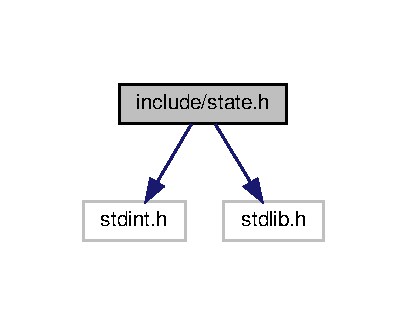
\includegraphics[width=196pt]{state_8h__incl}
\end{center}
\end{figure}
This graph shows which files directly or indirectly include this file\+:
\nopagebreak
\begin{figure}[H]
\begin{center}
\leavevmode
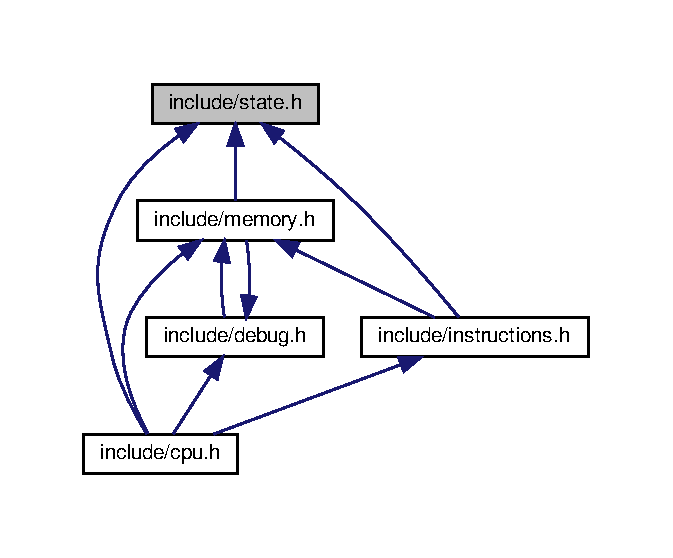
\includegraphics[width=323pt]{state_8h__dep__incl}
\end{center}
\end{figure}
\subsection*{Macros}
\begin{DoxyCompactItemize}
\item 
\#define \hyperlink{state_8h_a3e2525931bbdb2a18120b22f99c58fa0}{M\+O\+D\+E\+\_\+\+R\+UN}~0
\item 
\#define \hyperlink{state_8h_a9c2557a2d56dadc57824c046b0238a8d}{M\+O\+D\+E\+\_\+\+H\+A\+LT}~1
\item 
\#define \hyperlink{state_8h_a29a7dfd4fec0d672f9690159d70abc0d}{M\+O\+D\+E\+\_\+\+S\+T\+OP}~2
\end{DoxyCompactItemize}
\subsection*{Functions}
\begin{DoxyCompactItemize}
\item 
\mbox{\Hypertarget{state_8h_a8aac6477340919fc5e0dcd7ec8efa049}\label{state_8h_a8aac6477340919fc5e0dcd7ec8efa049}} 
void \hyperlink{state_8h_a8aac6477340919fc5e0dcd7ec8efa049}{State\+\_\+init} (void)
\begin{DoxyCompactList}\small\item\em Initialize the state of the emulator (registers, C\+PU mode, flags). \end{DoxyCompactList}\item 
uint8\+\_\+t \hyperlink{state_8h_ae1658eac5102fd259c5b22dd458cbab2}{Extract\+\_\+\+M\+SB} (uint16\+\_\+t i)
\begin{DoxyCompactList}\small\item\em Extract the most significant byte of an unsigned 16-\/bit constant. \end{DoxyCompactList}\item 
uint8\+\_\+t \hyperlink{state_8h_aad7eb305fc11715b17a900da0b0e6de3}{Extract\+\_\+\+L\+SB} (uint16\+\_\+t i)
\begin{DoxyCompactList}\small\item\em Extract the least significant byte of an unsigned 16-\/bit constant. \end{DoxyCompactList}\item 
uint16\+\_\+t \hyperlink{state_8h_ab085e353d471dd986e66ac71c78b51cb}{Combine\+\_\+\+M\+S\+B\+\_\+\+L\+SB} (uint8\+\_\+t msb, uint8\+\_\+t lsb)
\begin{DoxyCompactList}\small\item\em Combine two unsigned bytes into an unsigned 16-\/bit value. \end{DoxyCompactList}\item 
\mbox{\Hypertarget{state_8h_a7b158fb74f4b38a7661d9d325d8f7d11}\label{state_8h_a7b158fb74f4b38a7661d9d325d8f7d11}} 
void \hyperlink{state_8h_a7b158fb74f4b38a7661d9d325d8f7d11}{Registers\+\_\+init} (void)
\begin{DoxyCompactList}\small\item\em Initialize the values of the C\+PU registers. \end{DoxyCompactList}\item 
void \hyperlink{state_8h_a5bf0ec85d0c105ebf7178fab679fd4f8}{Flag\+\_\+set\+\_\+Z} (uint8\+\_\+t state)
\begin{DoxyCompactList}\small\item\em Set the Z-\/flag to a given value (0 or 1). \end{DoxyCompactList}\item 
void \hyperlink{state_8h_ac3257fc4c9a2319f178c6b7c50def4ff}{Flag\+\_\+set\+\_\+N} (uint8\+\_\+t state)
\begin{DoxyCompactList}\small\item\em Set the N-\/flag to a given value (0 or 1). \end{DoxyCompactList}\item 
void \hyperlink{state_8h_a34ac5640d5e81eb53acebbc77da56a42}{Flag\+\_\+set\+\_\+H} (uint8\+\_\+t state)
\begin{DoxyCompactList}\small\item\em Set the H-\/flag to a given value (0 or 1). \end{DoxyCompactList}\item 
void \hyperlink{state_8h_ac0e31fc044bf31edeb5d9c86a51f21c1}{Flag\+\_\+set\+\_\+C} (uint8\+\_\+t state)
\begin{DoxyCompactList}\small\item\em Set the C-\/flag to a given value (0 or 1). \end{DoxyCompactList}\item 
void \hyperlink{state_8h_afa8b8ce9d52e0f0efe0bac091698c4ef}{Flags\+\_\+set} (uint8\+\_\+t Z, uint8\+\_\+t N, uint8\+\_\+t \hyperlink{state_8h_ad1ee63aa0c7c876954eb9f5de083019e}{H}, uint8\+\_\+t \hyperlink{state_8h_a6f32a714c227b07e27db3e599edb419a}{C})
\begin{DoxyCompactList}\small\item\em Set the flags in the F-\/register to given values (0 = reset, 1 = set, -\/1 = don\textquotesingle{}t care). \end{DoxyCompactList}\item 
uint8\+\_\+t \hyperlink{state_8h_a0cce733f8bea02487ba45b18819ba948}{Flag\+\_\+test\+\_\+\+H\+\_\+\+U8\+\_\+\+U8} (uint8\+\_\+t a, uint8\+\_\+t b, uint8\+\_\+t add)
\begin{DoxyCompactList}\small\item\em Test for a halfcarry in the addition or substraction of two unsigned 8-\/bit constants. \end{DoxyCompactList}\item 
uint8\+\_\+t \hyperlink{state_8h_ae9c8132a81265c1acc16ad2d9a7570e2}{Flag\+\_\+test\+\_\+\+C\+\_\+\+U8\+\_\+\+U8} (uint8\+\_\+t a, uint8\+\_\+t b, uint8\+\_\+t add)
\begin{DoxyCompactList}\small\item\em Test for a carry in the addition or substraction of two unsigned 8-\/bit constants. \end{DoxyCompactList}\item 
uint8\+\_\+t \hyperlink{state_8h_a419f0e14d7e5c7edd095e346b7f776f1}{Flag\+\_\+test\+\_\+\+H\+\_\+\+U16\+\_\+\+S8} (uint16\+\_\+t a, int8\+\_\+t b)
\begin{DoxyCompactList}\small\item\em Test for a halfcarry (bit 11 to 12) in the addition an unsigned 16-\/bit constant and a signed 8-\/bit constant. \end{DoxyCompactList}\item 
uint8\+\_\+t \hyperlink{state_8h_a0e9a28936c367672398e75e5d6bdecc2}{Flag\+\_\+test\+\_\+\+C\+\_\+\+U16\+\_\+\+S8} (uint16\+\_\+t a, int8\+\_\+t b)
\begin{DoxyCompactList}\small\item\em Test for a carry (bit 15 to \char`\"{}16\char`\"{}) in the addition an unsigned 16-\/bit constant and a signed 8-\/bit constant. \end{DoxyCompactList}\item 
uint8\+\_\+t \hyperlink{state_8h_afeb5c65d472c8591aa13f8bc4ca10156}{Flag\+\_\+test\+\_\+\+H\+\_\+\+U16\+\_\+\+U16} (uint16\+\_\+t a, uint16\+\_\+t b)
\begin{DoxyCompactList}\small\item\em Test for a halfcarry in the addition of two unsigned 16-\/bit constants. \end{DoxyCompactList}\item 
uint8\+\_\+t \hyperlink{state_8h_add4dc6d2971b7af986e56752f1893c84}{Flag\+\_\+test\+\_\+\+C\+\_\+\+U16\+\_\+\+U16} (uint16\+\_\+t a, uint16\+\_\+t b)
\begin{DoxyCompactList}\small\item\em Test for a carry in the addition of two unsigned 16-\/bit constants. \end{DoxyCompactList}\item 
uint8\+\_\+t \hyperlink{state_8h_addd76f2cd1501b28589bfdba3f88db67}{Flag\+\_\+get\+\_\+Z} (void)
\begin{DoxyCompactList}\small\item\em Return the value of the Z-\/flag. \end{DoxyCompactList}\item 
uint8\+\_\+t \hyperlink{state_8h_a6cecaf76981f0c46fcd0103b0c949122}{Flag\+\_\+get\+\_\+N} (void)
\begin{DoxyCompactList}\small\item\em Return the value of the N-\/flag. \end{DoxyCompactList}\item 
uint8\+\_\+t \hyperlink{state_8h_a75b65cf0d75aa7958ff130ea5c0776c6}{Flag\+\_\+get\+\_\+H} (void)
\begin{DoxyCompactList}\small\item\em Return the value of the H-\/flag. \end{DoxyCompactList}\item 
uint8\+\_\+t \hyperlink{state_8h_a19a5d12cc5cc96fe31eecc5083ded92b}{Flag\+\_\+get\+\_\+C} (void)
\begin{DoxyCompactList}\small\item\em Return the value of the C-\/flag. \end{DoxyCompactList}\end{DoxyCompactItemize}
\subsection*{Variables}
\begin{DoxyCompactItemize}
\item 
\mbox{\Hypertarget{state_8h_ad6091a0e38f03b2c6c12aabb4b6cc59c}\label{state_8h_ad6091a0e38f03b2c6c12aabb4b6cc59c}} 
\begin{tabbing}
xx\=xx\=xx\=xx\=xx\=xx\=xx\=xx\=xx\=\kill
struct \{\\
\>uint8\_t \hyperlink{state_8h_a37e90f5e3bd99fac2021fb3a326607d4}{mode}\\
\>uint8\_t \hyperlink{state_8h_a3f404c2042eccd597794adcd3ed49b71}{IME}\\
\} \hyperlink{state_8h_ad6091a0e38f03b2c6c12aabb4b6cc59c}{State}\\

\end{tabbing}\begin{DoxyCompactList}\small\item\em Struct that represents the state of the C\+PU. \end{DoxyCompactList}\item 
\mbox{\Hypertarget{state_8h_a95fb456db5026d0f69e7e5698315fb9b}\label{state_8h_a95fb456db5026d0f69e7e5698315fb9b}} 
\begin{tabbing}
xx\=xx\=xx\=xx\=xx\=xx\=xx\=xx\=xx\=\kill
struct \{\\
\>char \hyperlink{state_8h_af984635a558e22d4669b0f9ee1298779}{name} \mbox{[}17\mbox{]}\\
\>uint8\_t \hyperlink{state_8h_a08ba47209d827a8cf708f2e7679fd020}{CGB\_flag}\\
\>uint8\_t \hyperlink{state_8h_ac56c83510a89c5469ffee4badabd2224}{cartridge\_type}\\
\>uint8\_t \hyperlink{state_8h_ad4bba274c31c57713318a5de8e18b0d2}{ROM\_size}\\
\>uint8\_t \hyperlink{state_8h_a200beecf76d43fb8dded424af571a0ee}{RAM\_size}\\
\>uint8\_t \hyperlink{state_8h_a42676c2cae17bc2fa151feea9e192342}{destination}\\
\} \hyperlink{state_8h_a95fb456db5026d0f69e7e5698315fb9b}{Cartridge}\\

\end{tabbing}\begin{DoxyCompactList}\small\item\em Struct that holds data from the cartridge header. \end{DoxyCompactList}\item 
\mbox{\Hypertarget{state_8h_a9418de733657f6fb1dc6fcc5c774abf8}\label{state_8h_a9418de733657f6fb1dc6fcc5c774abf8}} 
\begin{tabbing}
xx\=xx\=xx\=xx\=xx\=xx\=xx\=xx\=xx\=\kill
struct \{\\
\mbox{\Hypertarget{struct_0D8_ab84d627d679f68b687243dbc251e1d43}\label{struct_0D8_ab84d627d679f68b687243dbc251e1d43}} 
\>union \{\\
\mbox{\Hypertarget{union_0D8_1_1_0D9_a8c3b21f1b7099b4b36bc1c9643f78716}\label{union_0D8_1_1_0D9_a8c3b21f1b7099b4b36bc1c9643f78716}} 
\>\>struct \{\\
\>\>\>uint8\_t \hyperlink{state_8h_a576f877ccc2837ffe5811406404acad1}{F}\\
\>\>\>uint8\_t \hyperlink{state_8h_aa99de428bd3e7715b73b335a5af9e900}{A}\\
\>\>\} \\
\>\>uint16\_t \hyperlink{state_8h_a6e982288432855089a4873f7e10782c6}{AF}\\
\>\} \\
\mbox{\Hypertarget{struct_0D8_a037238800153f3a46b4cfbacb33285dd}\label{struct_0D8_a037238800153f3a46b4cfbacb33285dd}} 
\>union \{\\
\mbox{\Hypertarget{union_0D8_1_1_0D11_a8db5ad1450b4a3c4e4dacec2f2b2f946}\label{union_0D8_1_1_0D11_a8db5ad1450b4a3c4e4dacec2f2b2f946}} 
\>\>struct \{\\
\>\>\>uint8\_t \hyperlink{state_8h_a6f32a714c227b07e27db3e599edb419a}{C}\\
\>\>\>uint8\_t \hyperlink{state_8h_a7c7fb36d372d349a62c14f1e6c7337ea}{B}\\
\>\>\} \\
\>\>uint16\_t \hyperlink{state_8h_ad14ee14a830760900b01ab060e27761e}{BC}\\
\>\} \\
\mbox{\Hypertarget{struct_0D8_aeca95e7985fa62bbffe170f0ae8794e5}\label{struct_0D8_aeca95e7985fa62bbffe170f0ae8794e5}} 
\>union \{\\
\mbox{\Hypertarget{union_0D8_1_1_0D13_a4441399b81a9eae47fcef9a23b467a21}\label{union_0D8_1_1_0D13_a4441399b81a9eae47fcef9a23b467a21}} 
\>\>struct \{\\
\>\>\>uint8\_t \hyperlink{state_8h_a5866c444a2a78211eef583f48cd36225}{E}\\
\>\>\>uint8\_t \hyperlink{state_8h_a42ede28e876dcdb2ce2ddd730de0401e}{D}\\
\>\>\} \\
\>\>uint16\_t \hyperlink{state_8h_a076d7e0a7cd08a42568444b2fe643107}{DE}\\
\>\} \\
\mbox{\Hypertarget{struct_0D8_a4b95f08895d6e47dfdbd463eb889fcdf}\label{struct_0D8_a4b95f08895d6e47dfdbd463eb889fcdf}} 
\>union \{\\
\mbox{\Hypertarget{union_0D8_1_1_0D15_a3b3b3445a872750cd39aa42e608391a5}\label{union_0D8_1_1_0D15_a3b3b3445a872750cd39aa42e608391a5}} 
\>\>struct \{\\
\>\>\>uint8\_t \hyperlink{state_8h_aee73cc056696e504430c53eaa9c58cf0}{L}\\
\>\>\>uint8\_t \hyperlink{state_8h_ad1ee63aa0c7c876954eb9f5de083019e}{H}\\
\>\>\} \\
\>\>uint16\_t \hyperlink{state_8h_a35a5e2db4cabdc4c4d67d20b6d5169cf}{HL}\\
\>\} \\
\>uint16\_t \hyperlink{state_8h_a6381d5cc0641c44d5f9510e29a74fa16}{SP}\\
\>uint16\_t \hyperlink{state_8h_afa06037aaac5044b97dde7b9f8771ce6}{PC}\\
\} \hyperlink{state_8h_a9418de733657f6fb1dc6fcc5c774abf8}{Registers}\\

\end{tabbing}\begin{DoxyCompactList}\small\item\em Struct that holds the C\+PU registers. \end{DoxyCompactList}\end{DoxyCompactItemize}


\subsection{Detailed Description}
Representation of the state of the emulator (registers, C\+PU mode, flags) and a set of utility functions. 

\begin{DoxyAuthor}{Author}
tbnbooij 
\end{DoxyAuthor}
\begin{DoxyDate}{Date}
2018-\/08-\/13 
\end{DoxyDate}


\subsection{Macro Definition Documentation}
\mbox{\Hypertarget{state_8h_a9c2557a2d56dadc57824c046b0238a8d}\label{state_8h_a9c2557a2d56dadc57824c046b0238a8d}} 
\index{state.\+h@{state.\+h}!M\+O\+D\+E\+\_\+\+H\+A\+LT@{M\+O\+D\+E\+\_\+\+H\+A\+LT}}
\index{M\+O\+D\+E\+\_\+\+H\+A\+LT@{M\+O\+D\+E\+\_\+\+H\+A\+LT}!state.\+h@{state.\+h}}
\subsubsection{\texorpdfstring{M\+O\+D\+E\+\_\+\+H\+A\+LT}{MODE\_HALT}}
{\footnotesize\ttfamily \#define M\+O\+D\+E\+\_\+\+H\+A\+LT~1}

C\+PU mode 1\+: Halt; Power down C\+PU until an interrupt occurs (reduce power consumption) \mbox{\Hypertarget{state_8h_a3e2525931bbdb2a18120b22f99c58fa0}\label{state_8h_a3e2525931bbdb2a18120b22f99c58fa0}} 
\index{state.\+h@{state.\+h}!M\+O\+D\+E\+\_\+\+R\+UN@{M\+O\+D\+E\+\_\+\+R\+UN}}
\index{M\+O\+D\+E\+\_\+\+R\+UN@{M\+O\+D\+E\+\_\+\+R\+UN}!state.\+h@{state.\+h}}
\subsubsection{\texorpdfstring{M\+O\+D\+E\+\_\+\+R\+UN}{MODE\_RUN}}
{\footnotesize\ttfamily \#define M\+O\+D\+E\+\_\+\+R\+UN~0}

C\+PU mode 0\+: Running \mbox{\Hypertarget{state_8h_a29a7dfd4fec0d672f9690159d70abc0d}\label{state_8h_a29a7dfd4fec0d672f9690159d70abc0d}} 
\index{state.\+h@{state.\+h}!M\+O\+D\+E\+\_\+\+S\+T\+OP@{M\+O\+D\+E\+\_\+\+S\+T\+OP}}
\index{M\+O\+D\+E\+\_\+\+S\+T\+OP@{M\+O\+D\+E\+\_\+\+S\+T\+OP}!state.\+h@{state.\+h}}
\subsubsection{\texorpdfstring{M\+O\+D\+E\+\_\+\+S\+T\+OP}{MODE\_STOP}}
{\footnotesize\ttfamily \#define M\+O\+D\+E\+\_\+\+S\+T\+OP~2}

C\+PU mode 2\+: Stop; Halt C\+PU and L\+CD display until a button is pressed 

\subsection{Function Documentation}
\mbox{\Hypertarget{state_8h_ab085e353d471dd986e66ac71c78b51cb}\label{state_8h_ab085e353d471dd986e66ac71c78b51cb}} 
\index{state.\+h@{state.\+h}!Combine\+\_\+\+M\+S\+B\+\_\+\+L\+SB@{Combine\+\_\+\+M\+S\+B\+\_\+\+L\+SB}}
\index{Combine\+\_\+\+M\+S\+B\+\_\+\+L\+SB@{Combine\+\_\+\+M\+S\+B\+\_\+\+L\+SB}!state.\+h@{state.\+h}}
\subsubsection{\texorpdfstring{Combine\+\_\+\+M\+S\+B\+\_\+\+L\+S\+B()}{Combine\_MSB\_LSB()}}
{\footnotesize\ttfamily uint16\+\_\+t Combine\+\_\+\+M\+S\+B\+\_\+\+L\+SB (\begin{DoxyParamCaption}\item[{uint8\+\_\+t}]{msb,  }\item[{uint8\+\_\+t}]{lsb }\end{DoxyParamCaption})}



Combine two unsigned bytes into an unsigned 16-\/bit value. 


\begin{DoxyParams}{Parameters}
{\em msb} & The most significant byte \\
\hline
{\em lsb} & The least significant byte \\
\hline
\end{DoxyParams}
\begin{DoxyReturn}{Returns}
uint16\+\_\+t The combination of the two input bytes 
\end{DoxyReturn}
\mbox{\Hypertarget{state_8h_aad7eb305fc11715b17a900da0b0e6de3}\label{state_8h_aad7eb305fc11715b17a900da0b0e6de3}} 
\index{state.\+h@{state.\+h}!Extract\+\_\+\+L\+SB@{Extract\+\_\+\+L\+SB}}
\index{Extract\+\_\+\+L\+SB@{Extract\+\_\+\+L\+SB}!state.\+h@{state.\+h}}
\subsubsection{\texorpdfstring{Extract\+\_\+\+L\+S\+B()}{Extract\_LSB()}}
{\footnotesize\ttfamily uint8\+\_\+t Extract\+\_\+\+L\+SB (\begin{DoxyParamCaption}\item[{uint16\+\_\+t}]{i }\end{DoxyParamCaption})}



Extract the least significant byte of an unsigned 16-\/bit constant. 


\begin{DoxyParams}{Parameters}
{\em i} & Unsigned 16-\/bit constant \\
\hline
\end{DoxyParams}
\begin{DoxyReturn}{Returns}
uint8\+\_\+t The least significant byte of i 
\end{DoxyReturn}
\mbox{\Hypertarget{state_8h_ae1658eac5102fd259c5b22dd458cbab2}\label{state_8h_ae1658eac5102fd259c5b22dd458cbab2}} 
\index{state.\+h@{state.\+h}!Extract\+\_\+\+M\+SB@{Extract\+\_\+\+M\+SB}}
\index{Extract\+\_\+\+M\+SB@{Extract\+\_\+\+M\+SB}!state.\+h@{state.\+h}}
\subsubsection{\texorpdfstring{Extract\+\_\+\+M\+S\+B()}{Extract\_MSB()}}
{\footnotesize\ttfamily uint8\+\_\+t Extract\+\_\+\+M\+SB (\begin{DoxyParamCaption}\item[{uint16\+\_\+t}]{i }\end{DoxyParamCaption})}



Extract the most significant byte of an unsigned 16-\/bit constant. 


\begin{DoxyParams}{Parameters}
{\em i} & Unsigned 16-\/bit constant \\
\hline
\end{DoxyParams}
\begin{DoxyReturn}{Returns}
uint8\+\_\+t The most significant byte of i 
\end{DoxyReturn}
\mbox{\Hypertarget{state_8h_a19a5d12cc5cc96fe31eecc5083ded92b}\label{state_8h_a19a5d12cc5cc96fe31eecc5083ded92b}} 
\index{state.\+h@{state.\+h}!Flag\+\_\+get\+\_\+C@{Flag\+\_\+get\+\_\+C}}
\index{Flag\+\_\+get\+\_\+C@{Flag\+\_\+get\+\_\+C}!state.\+h@{state.\+h}}
\subsubsection{\texorpdfstring{Flag\+\_\+get\+\_\+\+C()}{Flag\_get\_C()}}
{\footnotesize\ttfamily uint8\+\_\+t Flag\+\_\+get\+\_\+C (\begin{DoxyParamCaption}\item[{void}]{ }\end{DoxyParamCaption})}



Return the value of the C-\/flag. 

\begin{DoxyReturn}{Returns}
uint8\+\_\+t The value of the C-\/flag 
\end{DoxyReturn}
\mbox{\Hypertarget{state_8h_a75b65cf0d75aa7958ff130ea5c0776c6}\label{state_8h_a75b65cf0d75aa7958ff130ea5c0776c6}} 
\index{state.\+h@{state.\+h}!Flag\+\_\+get\+\_\+H@{Flag\+\_\+get\+\_\+H}}
\index{Flag\+\_\+get\+\_\+H@{Flag\+\_\+get\+\_\+H}!state.\+h@{state.\+h}}
\subsubsection{\texorpdfstring{Flag\+\_\+get\+\_\+\+H()}{Flag\_get\_H()}}
{\footnotesize\ttfamily uint8\+\_\+t Flag\+\_\+get\+\_\+H (\begin{DoxyParamCaption}\item[{void}]{ }\end{DoxyParamCaption})}



Return the value of the H-\/flag. 

\begin{DoxyReturn}{Returns}
uint8\+\_\+t The value of the H-\/flag 
\end{DoxyReturn}
\mbox{\Hypertarget{state_8h_a6cecaf76981f0c46fcd0103b0c949122}\label{state_8h_a6cecaf76981f0c46fcd0103b0c949122}} 
\index{state.\+h@{state.\+h}!Flag\+\_\+get\+\_\+N@{Flag\+\_\+get\+\_\+N}}
\index{Flag\+\_\+get\+\_\+N@{Flag\+\_\+get\+\_\+N}!state.\+h@{state.\+h}}
\subsubsection{\texorpdfstring{Flag\+\_\+get\+\_\+\+N()}{Flag\_get\_N()}}
{\footnotesize\ttfamily uint8\+\_\+t Flag\+\_\+get\+\_\+N (\begin{DoxyParamCaption}\item[{void}]{ }\end{DoxyParamCaption})}



Return the value of the N-\/flag. 

\begin{DoxyReturn}{Returns}
uint8\+\_\+t The value of the N-\/flag 
\end{DoxyReturn}
\mbox{\Hypertarget{state_8h_addd76f2cd1501b28589bfdba3f88db67}\label{state_8h_addd76f2cd1501b28589bfdba3f88db67}} 
\index{state.\+h@{state.\+h}!Flag\+\_\+get\+\_\+Z@{Flag\+\_\+get\+\_\+Z}}
\index{Flag\+\_\+get\+\_\+Z@{Flag\+\_\+get\+\_\+Z}!state.\+h@{state.\+h}}
\subsubsection{\texorpdfstring{Flag\+\_\+get\+\_\+\+Z()}{Flag\_get\_Z()}}
{\footnotesize\ttfamily uint8\+\_\+t Flag\+\_\+get\+\_\+Z (\begin{DoxyParamCaption}\item[{void}]{ }\end{DoxyParamCaption})}



Return the value of the Z-\/flag. 

\begin{DoxyReturn}{Returns}
uint8\+\_\+t The value of the Z-\/flag 
\end{DoxyReturn}
\mbox{\Hypertarget{state_8h_ac0e31fc044bf31edeb5d9c86a51f21c1}\label{state_8h_ac0e31fc044bf31edeb5d9c86a51f21c1}} 
\index{state.\+h@{state.\+h}!Flag\+\_\+set\+\_\+C@{Flag\+\_\+set\+\_\+C}}
\index{Flag\+\_\+set\+\_\+C@{Flag\+\_\+set\+\_\+C}!state.\+h@{state.\+h}}
\subsubsection{\texorpdfstring{Flag\+\_\+set\+\_\+\+C()}{Flag\_set\_C()}}
{\footnotesize\ttfamily void Flag\+\_\+set\+\_\+C (\begin{DoxyParamCaption}\item[{uint8\+\_\+t}]{state }\end{DoxyParamCaption})}



Set the C-\/flag to a given value (0 or 1). 


\begin{DoxyParams}{Parameters}
{\em state} & The state (0 or 1) that the C-\/flag is set to \\
\hline
\end{DoxyParams}
\mbox{\Hypertarget{state_8h_a34ac5640d5e81eb53acebbc77da56a42}\label{state_8h_a34ac5640d5e81eb53acebbc77da56a42}} 
\index{state.\+h@{state.\+h}!Flag\+\_\+set\+\_\+H@{Flag\+\_\+set\+\_\+H}}
\index{Flag\+\_\+set\+\_\+H@{Flag\+\_\+set\+\_\+H}!state.\+h@{state.\+h}}
\subsubsection{\texorpdfstring{Flag\+\_\+set\+\_\+\+H()}{Flag\_set\_H()}}
{\footnotesize\ttfamily void Flag\+\_\+set\+\_\+H (\begin{DoxyParamCaption}\item[{uint8\+\_\+t}]{state }\end{DoxyParamCaption})}



Set the H-\/flag to a given value (0 or 1). 


\begin{DoxyParams}{Parameters}
{\em state} & The state (0 or 1) that the H-\/flag is set to \\
\hline
\end{DoxyParams}
\mbox{\Hypertarget{state_8h_ac3257fc4c9a2319f178c6b7c50def4ff}\label{state_8h_ac3257fc4c9a2319f178c6b7c50def4ff}} 
\index{state.\+h@{state.\+h}!Flag\+\_\+set\+\_\+N@{Flag\+\_\+set\+\_\+N}}
\index{Flag\+\_\+set\+\_\+N@{Flag\+\_\+set\+\_\+N}!state.\+h@{state.\+h}}
\subsubsection{\texorpdfstring{Flag\+\_\+set\+\_\+\+N()}{Flag\_set\_N()}}
{\footnotesize\ttfamily void Flag\+\_\+set\+\_\+N (\begin{DoxyParamCaption}\item[{uint8\+\_\+t}]{state }\end{DoxyParamCaption})}



Set the N-\/flag to a given value (0 or 1). 


\begin{DoxyParams}{Parameters}
{\em state} & The state (0 or 1) that the N-\/flag is set to \\
\hline
\end{DoxyParams}
\mbox{\Hypertarget{state_8h_a5bf0ec85d0c105ebf7178fab679fd4f8}\label{state_8h_a5bf0ec85d0c105ebf7178fab679fd4f8}} 
\index{state.\+h@{state.\+h}!Flag\+\_\+set\+\_\+Z@{Flag\+\_\+set\+\_\+Z}}
\index{Flag\+\_\+set\+\_\+Z@{Flag\+\_\+set\+\_\+Z}!state.\+h@{state.\+h}}
\subsubsection{\texorpdfstring{Flag\+\_\+set\+\_\+\+Z()}{Flag\_set\_Z()}}
{\footnotesize\ttfamily void Flag\+\_\+set\+\_\+Z (\begin{DoxyParamCaption}\item[{uint8\+\_\+t}]{state }\end{DoxyParamCaption})}



Set the Z-\/flag to a given value (0 or 1). 


\begin{DoxyParams}{Parameters}
{\em state} & The state (0 or 1) that the Z-\/flag is set to \\
\hline
\end{DoxyParams}
\mbox{\Hypertarget{state_8h_a0e9a28936c367672398e75e5d6bdecc2}\label{state_8h_a0e9a28936c367672398e75e5d6bdecc2}} 
\index{state.\+h@{state.\+h}!Flag\+\_\+test\+\_\+\+C\+\_\+\+U16\+\_\+\+S8@{Flag\+\_\+test\+\_\+\+C\+\_\+\+U16\+\_\+\+S8}}
\index{Flag\+\_\+test\+\_\+\+C\+\_\+\+U16\+\_\+\+S8@{Flag\+\_\+test\+\_\+\+C\+\_\+\+U16\+\_\+\+S8}!state.\+h@{state.\+h}}
\subsubsection{\texorpdfstring{Flag\+\_\+test\+\_\+\+C\+\_\+\+U16\+\_\+\+S8()}{Flag\_test\_C\_U16\_S8()}}
{\footnotesize\ttfamily uint8\+\_\+t Flag\+\_\+test\+\_\+\+C\+\_\+\+U16\+\_\+\+S8 (\begin{DoxyParamCaption}\item[{uint16\+\_\+t}]{a,  }\item[{int8\+\_\+t}]{b }\end{DoxyParamCaption})}



Test for a carry (bit 15 to \char`\"{}16\char`\"{}) in the addition an unsigned 16-\/bit constant and a signed 8-\/bit constant. 


\begin{DoxyParams}{Parameters}
{\em a} & Unsigned 16-\/bit constant \\
\hline
{\em b} & Signed 8-\/bit constant \\
\hline
\end{DoxyParams}
\begin{DoxyReturn}{Returns}
uint8\+\_\+t Boolean that represents whether a carry occurs or not 
\end{DoxyReturn}
\mbox{\Hypertarget{state_8h_add4dc6d2971b7af986e56752f1893c84}\label{state_8h_add4dc6d2971b7af986e56752f1893c84}} 
\index{state.\+h@{state.\+h}!Flag\+\_\+test\+\_\+\+C\+\_\+\+U16\+\_\+\+U16@{Flag\+\_\+test\+\_\+\+C\+\_\+\+U16\+\_\+\+U16}}
\index{Flag\+\_\+test\+\_\+\+C\+\_\+\+U16\+\_\+\+U16@{Flag\+\_\+test\+\_\+\+C\+\_\+\+U16\+\_\+\+U16}!state.\+h@{state.\+h}}
\subsubsection{\texorpdfstring{Flag\+\_\+test\+\_\+\+C\+\_\+\+U16\+\_\+\+U16()}{Flag\_test\_C\_U16\_U16()}}
{\footnotesize\ttfamily uint8\+\_\+t Flag\+\_\+test\+\_\+\+C\+\_\+\+U16\+\_\+\+U16 (\begin{DoxyParamCaption}\item[{uint16\+\_\+t}]{a,  }\item[{uint16\+\_\+t}]{b }\end{DoxyParamCaption})}



Test for a carry in the addition of two unsigned 16-\/bit constants. 


\begin{DoxyParams}{Parameters}
{\em a} & Unsigned 16-\/bit constant \\
\hline
{\em b} & Unsigned 16-\/bit constant \\
\hline
\end{DoxyParams}
\begin{DoxyReturn}{Returns}
uint8\+\_\+t Boolean that represents whether a carry occurs or not 
\end{DoxyReturn}
\mbox{\Hypertarget{state_8h_ae9c8132a81265c1acc16ad2d9a7570e2}\label{state_8h_ae9c8132a81265c1acc16ad2d9a7570e2}} 
\index{state.\+h@{state.\+h}!Flag\+\_\+test\+\_\+\+C\+\_\+\+U8\+\_\+\+U8@{Flag\+\_\+test\+\_\+\+C\+\_\+\+U8\+\_\+\+U8}}
\index{Flag\+\_\+test\+\_\+\+C\+\_\+\+U8\+\_\+\+U8@{Flag\+\_\+test\+\_\+\+C\+\_\+\+U8\+\_\+\+U8}!state.\+h@{state.\+h}}
\subsubsection{\texorpdfstring{Flag\+\_\+test\+\_\+\+C\+\_\+\+U8\+\_\+\+U8()}{Flag\_test\_C\_U8\_U8()}}
{\footnotesize\ttfamily uint8\+\_\+t Flag\+\_\+test\+\_\+\+C\+\_\+\+U8\+\_\+\+U8 (\begin{DoxyParamCaption}\item[{uint8\+\_\+t}]{a,  }\item[{uint8\+\_\+t}]{b,  }\item[{uint8\+\_\+t}]{add }\end{DoxyParamCaption})}



Test for a carry in the addition or substraction of two unsigned 8-\/bit constants. 


\begin{DoxyParams}{Parameters}
{\em a} & Unsigned 8-\/bit constant \\
\hline
{\em b} & Unsigned 8-\/bit constant \\
\hline
{\em add} & The operation that is applied to the two constants (subtraction = 0, addition = 1) \\
\hline
\end{DoxyParams}
\begin{DoxyReturn}{Returns}
uint8\+\_\+t Boolean that represents whether a carry occurs or not 
\end{DoxyReturn}
\mbox{\Hypertarget{state_8h_a419f0e14d7e5c7edd095e346b7f776f1}\label{state_8h_a419f0e14d7e5c7edd095e346b7f776f1}} 
\index{state.\+h@{state.\+h}!Flag\+\_\+test\+\_\+\+H\+\_\+\+U16\+\_\+\+S8@{Flag\+\_\+test\+\_\+\+H\+\_\+\+U16\+\_\+\+S8}}
\index{Flag\+\_\+test\+\_\+\+H\+\_\+\+U16\+\_\+\+S8@{Flag\+\_\+test\+\_\+\+H\+\_\+\+U16\+\_\+\+S8}!state.\+h@{state.\+h}}
\subsubsection{\texorpdfstring{Flag\+\_\+test\+\_\+\+H\+\_\+\+U16\+\_\+\+S8()}{Flag\_test\_H\_U16\_S8()}}
{\footnotesize\ttfamily uint8\+\_\+t Flag\+\_\+test\+\_\+\+H\+\_\+\+U16\+\_\+\+S8 (\begin{DoxyParamCaption}\item[{uint16\+\_\+t}]{a,  }\item[{int8\+\_\+t}]{b }\end{DoxyParamCaption})}



Test for a halfcarry (bit 11 to 12) in the addition an unsigned 16-\/bit constant and a signed 8-\/bit constant. 


\begin{DoxyParams}{Parameters}
{\em a} & Unsigned 16-\/bit constant \\
\hline
{\em b} & Signed 8-\/bit constant \\
\hline
\end{DoxyParams}
\begin{DoxyReturn}{Returns}
uint8\+\_\+t Boolean that represents whether a halfcarry occurs or not 
\end{DoxyReturn}
\mbox{\Hypertarget{state_8h_afeb5c65d472c8591aa13f8bc4ca10156}\label{state_8h_afeb5c65d472c8591aa13f8bc4ca10156}} 
\index{state.\+h@{state.\+h}!Flag\+\_\+test\+\_\+\+H\+\_\+\+U16\+\_\+\+U16@{Flag\+\_\+test\+\_\+\+H\+\_\+\+U16\+\_\+\+U16}}
\index{Flag\+\_\+test\+\_\+\+H\+\_\+\+U16\+\_\+\+U16@{Flag\+\_\+test\+\_\+\+H\+\_\+\+U16\+\_\+\+U16}!state.\+h@{state.\+h}}
\subsubsection{\texorpdfstring{Flag\+\_\+test\+\_\+\+H\+\_\+\+U16\+\_\+\+U16()}{Flag\_test\_H\_U16\_U16()}}
{\footnotesize\ttfamily uint8\+\_\+t Flag\+\_\+test\+\_\+\+H\+\_\+\+U16\+\_\+\+U16 (\begin{DoxyParamCaption}\item[{uint16\+\_\+t}]{a,  }\item[{uint16\+\_\+t}]{b }\end{DoxyParamCaption})}



Test for a halfcarry in the addition of two unsigned 16-\/bit constants. 


\begin{DoxyParams}{Parameters}
{\em a} & Unsigned 16-\/bit constant \\
\hline
{\em b} & Unsigned 16-\/bit constant \\
\hline
\end{DoxyParams}
\begin{DoxyReturn}{Returns}
uint8\+\_\+t Boolean that represents whether a halfcarry occurs or not 
\end{DoxyReturn}
\mbox{\Hypertarget{state_8h_a0cce733f8bea02487ba45b18819ba948}\label{state_8h_a0cce733f8bea02487ba45b18819ba948}} 
\index{state.\+h@{state.\+h}!Flag\+\_\+test\+\_\+\+H\+\_\+\+U8\+\_\+\+U8@{Flag\+\_\+test\+\_\+\+H\+\_\+\+U8\+\_\+\+U8}}
\index{Flag\+\_\+test\+\_\+\+H\+\_\+\+U8\+\_\+\+U8@{Flag\+\_\+test\+\_\+\+H\+\_\+\+U8\+\_\+\+U8}!state.\+h@{state.\+h}}
\subsubsection{\texorpdfstring{Flag\+\_\+test\+\_\+\+H\+\_\+\+U8\+\_\+\+U8()}{Flag\_test\_H\_U8\_U8()}}
{\footnotesize\ttfamily uint8\+\_\+t Flag\+\_\+test\+\_\+\+H\+\_\+\+U8\+\_\+\+U8 (\begin{DoxyParamCaption}\item[{uint8\+\_\+t}]{a,  }\item[{uint8\+\_\+t}]{b,  }\item[{uint8\+\_\+t}]{add }\end{DoxyParamCaption})}



Test for a halfcarry in the addition or substraction of two unsigned 8-\/bit constants. 


\begin{DoxyParams}{Parameters}
{\em a} & Unsigned 8-\/bit constant \\
\hline
{\em b} & Unsigned 8-\/bit constant \\
\hline
{\em add} & The operation that is applied to the two constants (subtraction = 0, addition = 1) \\
\hline
\end{DoxyParams}
\begin{DoxyReturn}{Returns}
uint8\+\_\+t Boolean that represents whether a halfcarry occurs or not 
\end{DoxyReturn}
\mbox{\Hypertarget{state_8h_afa8b8ce9d52e0f0efe0bac091698c4ef}\label{state_8h_afa8b8ce9d52e0f0efe0bac091698c4ef}} 
\index{state.\+h@{state.\+h}!Flags\+\_\+set@{Flags\+\_\+set}}
\index{Flags\+\_\+set@{Flags\+\_\+set}!state.\+h@{state.\+h}}
\subsubsection{\texorpdfstring{Flags\+\_\+set()}{Flags\_set()}}
{\footnotesize\ttfamily void Flags\+\_\+set (\begin{DoxyParamCaption}\item[{uint8\+\_\+t}]{Z,  }\item[{uint8\+\_\+t}]{N,  }\item[{uint8\+\_\+t}]{H,  }\item[{uint8\+\_\+t}]{C }\end{DoxyParamCaption})}



Set the flags in the F-\/register to given values (0 = reset, 1 = set, -\/1 = don\textquotesingle{}t care). 


\begin{DoxyParams}{Parameters}
{\em Z} & The state (0/1/-\/1) that the Z-\/flag is set to \\
\hline
{\em N} & The state (0/1/-\/1) that the N-\/flag is set to \\
\hline
{\em H} & The state (0/1/-\/1) that the H-\/flag is set to \\
\hline
{\em C} & The state (0/1/-\/1) that the C-\/flag is set to \\
\hline
\end{DoxyParams}


\subsection{Variable Documentation}
\mbox{\Hypertarget{state_8h_aa99de428bd3e7715b73b335a5af9e900}\label{state_8h_aa99de428bd3e7715b73b335a5af9e900}} 
\index{state.\+h@{state.\+h}!A@{A}}
\index{A@{A}!state.\+h@{state.\+h}}
\subsubsection{\texorpdfstring{A}{A}}
{\footnotesize\ttfamily uint8\+\_\+t A}

8-\/bit accumulator register \mbox{\Hypertarget{state_8h_a6e982288432855089a4873f7e10782c6}\label{state_8h_a6e982288432855089a4873f7e10782c6}} 
\index{state.\+h@{state.\+h}!AF@{AF}}
\index{AF@{AF}!state.\+h@{state.\+h}}
\subsubsection{\texorpdfstring{AF}{AF}}
{\footnotesize\ttfamily uint16\+\_\+t AF}

16-\/bit general-\/purpose register \mbox{\Hypertarget{state_8h_a7c7fb36d372d349a62c14f1e6c7337ea}\label{state_8h_a7c7fb36d372d349a62c14f1e6c7337ea}} 
\index{state.\+h@{state.\+h}!B@{B}}
\index{B@{B}!state.\+h@{state.\+h}}
\subsubsection{\texorpdfstring{B}{B}}
{\footnotesize\ttfamily uint8\+\_\+t B}

8-\/bit general-\/purpose register \mbox{\Hypertarget{state_8h_ad14ee14a830760900b01ab060e27761e}\label{state_8h_ad14ee14a830760900b01ab060e27761e}} 
\index{state.\+h@{state.\+h}!BC@{BC}}
\index{BC@{BC}!state.\+h@{state.\+h}}
\subsubsection{\texorpdfstring{BC}{BC}}
{\footnotesize\ttfamily uint16\+\_\+t BC}

16-\/bit general-\/purpose register \mbox{\Hypertarget{state_8h_a6f32a714c227b07e27db3e599edb419a}\label{state_8h_a6f32a714c227b07e27db3e599edb419a}} 
\index{state.\+h@{state.\+h}!C@{C}}
\index{C@{C}!state.\+h@{state.\+h}}
\subsubsection{\texorpdfstring{C}{C}}
{\footnotesize\ttfamily uint8\+\_\+t C}

8-\/bit general-\/purpose register \mbox{\Hypertarget{state_8h_ac56c83510a89c5469ffee4badabd2224}\label{state_8h_ac56c83510a89c5469ffee4badabd2224}} 
\index{state.\+h@{state.\+h}!cartridge\+\_\+type@{cartridge\+\_\+type}}
\index{cartridge\+\_\+type@{cartridge\+\_\+type}!state.\+h@{state.\+h}}
\subsubsection{\texorpdfstring{cartridge\+\_\+type}{cartridge\_type}}
{\footnotesize\ttfamily uint8\+\_\+t cartridge\+\_\+type}

Flag that indicates the type of catridge (R\+OM, R\+AM, M\+BC, auxiliary hardware) \mbox{\Hypertarget{state_8h_a08ba47209d827a8cf708f2e7679fd020}\label{state_8h_a08ba47209d827a8cf708f2e7679fd020}} 
\index{state.\+h@{state.\+h}!C\+G\+B\+\_\+flag@{C\+G\+B\+\_\+flag}}
\index{C\+G\+B\+\_\+flag@{C\+G\+B\+\_\+flag}!state.\+h@{state.\+h}}
\subsubsection{\texorpdfstring{C\+G\+B\+\_\+flag}{CGB\_flag}}
{\footnotesize\ttfamily uint8\+\_\+t C\+G\+B\+\_\+flag}

Flag that indicates whether the cartridge was made for C\+GB (0x80) or D\+MG (0x00) \mbox{\Hypertarget{state_8h_a42ede28e876dcdb2ce2ddd730de0401e}\label{state_8h_a42ede28e876dcdb2ce2ddd730de0401e}} 
\index{state.\+h@{state.\+h}!D@{D}}
\index{D@{D}!state.\+h@{state.\+h}}
\subsubsection{\texorpdfstring{D}{D}}
{\footnotesize\ttfamily uint8\+\_\+t D}

8-\/bit general-\/purpose register \mbox{\Hypertarget{state_8h_a076d7e0a7cd08a42568444b2fe643107}\label{state_8h_a076d7e0a7cd08a42568444b2fe643107}} 
\index{state.\+h@{state.\+h}!DE@{DE}}
\index{DE@{DE}!state.\+h@{state.\+h}}
\subsubsection{\texorpdfstring{DE}{DE}}
{\footnotesize\ttfamily uint16\+\_\+t DE}

16-\/bit general-\/purpose register \mbox{\Hypertarget{state_8h_a42676c2cae17bc2fa151feea9e192342}\label{state_8h_a42676c2cae17bc2fa151feea9e192342}} 
\index{state.\+h@{state.\+h}!destination@{destination}}
\index{destination@{destination}!state.\+h@{state.\+h}}
\subsubsection{\texorpdfstring{destination}{destination}}
{\footnotesize\ttfamily uint8\+\_\+t destination}

Flag that indicates the destination the R\+OM was distributed to (0 = Japan, 1 = Outside of Japan) \mbox{\Hypertarget{state_8h_a5866c444a2a78211eef583f48cd36225}\label{state_8h_a5866c444a2a78211eef583f48cd36225}} 
\index{state.\+h@{state.\+h}!E@{E}}
\index{E@{E}!state.\+h@{state.\+h}}
\subsubsection{\texorpdfstring{E}{E}}
{\footnotesize\ttfamily uint8\+\_\+t E}

8-\/bit general-\/purpose register \mbox{\Hypertarget{state_8h_a576f877ccc2837ffe5811406404acad1}\label{state_8h_a576f877ccc2837ffe5811406404acad1}} 
\index{state.\+h@{state.\+h}!F@{F}}
\index{F@{F}!state.\+h@{state.\+h}}
\subsubsection{\texorpdfstring{F}{F}}
{\footnotesize\ttfamily uint8\+\_\+t F}

8-\/bit flags register \mbox{\Hypertarget{state_8h_ad1ee63aa0c7c876954eb9f5de083019e}\label{state_8h_ad1ee63aa0c7c876954eb9f5de083019e}} 
\index{state.\+h@{state.\+h}!H@{H}}
\index{H@{H}!state.\+h@{state.\+h}}
\subsubsection{\texorpdfstring{H}{H}}
{\footnotesize\ttfamily uint8\+\_\+t H}

8-\/bit general-\/purpose register \mbox{\Hypertarget{state_8h_a35a5e2db4cabdc4c4d67d20b6d5169cf}\label{state_8h_a35a5e2db4cabdc4c4d67d20b6d5169cf}} 
\index{state.\+h@{state.\+h}!HL@{HL}}
\index{HL@{HL}!state.\+h@{state.\+h}}
\subsubsection{\texorpdfstring{HL}{HL}}
{\footnotesize\ttfamily uint16\+\_\+t HL}

16-\/bit general-\/purpose register \mbox{\Hypertarget{state_8h_a3f404c2042eccd597794adcd3ed49b71}\label{state_8h_a3f404c2042eccd597794adcd3ed49b71}} 
\index{state.\+h@{state.\+h}!I\+ME@{I\+ME}}
\index{I\+ME@{I\+ME}!state.\+h@{state.\+h}}
\subsubsection{\texorpdfstring{I\+ME}{IME}}
{\footnotesize\ttfamily uint8\+\_\+t I\+ME}

Interrupt master enable (not to be confused with the interrupt enable register) \mbox{\Hypertarget{state_8h_aee73cc056696e504430c53eaa9c58cf0}\label{state_8h_aee73cc056696e504430c53eaa9c58cf0}} 
\index{state.\+h@{state.\+h}!L@{L}}
\index{L@{L}!state.\+h@{state.\+h}}
\subsubsection{\texorpdfstring{L}{L}}
{\footnotesize\ttfamily uint8\+\_\+t L}

8-\/bit general-\/purpose register \mbox{\Hypertarget{state_8h_a37e90f5e3bd99fac2021fb3a326607d4}\label{state_8h_a37e90f5e3bd99fac2021fb3a326607d4}} 
\index{state.\+h@{state.\+h}!mode@{mode}}
\index{mode@{mode}!state.\+h@{state.\+h}}
\subsubsection{\texorpdfstring{mode}{mode}}
{\footnotesize\ttfamily uint8\+\_\+t mode}

The mode in which the C\+PU is currently operating (run, halt, stop) \mbox{\Hypertarget{state_8h_af984635a558e22d4669b0f9ee1298779}\label{state_8h_af984635a558e22d4669b0f9ee1298779}} 
\index{state.\+h@{state.\+h}!name@{name}}
\index{name@{name}!state.\+h@{state.\+h}}
\subsubsection{\texorpdfstring{name}{name}}
{\footnotesize\ttfamily char name\mbox{[}17\mbox{]}}

The name of the cartridge in upper case A\+S\+C\+II \mbox{\Hypertarget{state_8h_afa06037aaac5044b97dde7b9f8771ce6}\label{state_8h_afa06037aaac5044b97dde7b9f8771ce6}} 
\index{state.\+h@{state.\+h}!PC@{PC}}
\index{PC@{PC}!state.\+h@{state.\+h}}
\subsubsection{\texorpdfstring{PC}{PC}}
{\footnotesize\ttfamily uint16\+\_\+t PC}

16-\/bit program counter \mbox{\Hypertarget{state_8h_a200beecf76d43fb8dded424af571a0ee}\label{state_8h_a200beecf76d43fb8dded424af571a0ee}} 
\index{state.\+h@{state.\+h}!R\+A\+M\+\_\+size@{R\+A\+M\+\_\+size}}
\index{R\+A\+M\+\_\+size@{R\+A\+M\+\_\+size}!state.\+h@{state.\+h}}
\subsubsection{\texorpdfstring{R\+A\+M\+\_\+size}{RAM\_size}}
{\footnotesize\ttfamily uint8\+\_\+t R\+A\+M\+\_\+size}

Flag that indicates the size of the additional R\+AM the cartridge contains \mbox{\Hypertarget{state_8h_ad4bba274c31c57713318a5de8e18b0d2}\label{state_8h_ad4bba274c31c57713318a5de8e18b0d2}} 
\index{state.\+h@{state.\+h}!R\+O\+M\+\_\+size@{R\+O\+M\+\_\+size}}
\index{R\+O\+M\+\_\+size@{R\+O\+M\+\_\+size}!state.\+h@{state.\+h}}
\subsubsection{\texorpdfstring{R\+O\+M\+\_\+size}{ROM\_size}}
{\footnotesize\ttfamily uint8\+\_\+t R\+O\+M\+\_\+size}

Flag that indicates the size of the R\+OM the cartridge holds \mbox{\Hypertarget{state_8h_a6381d5cc0641c44d5f9510e29a74fa16}\label{state_8h_a6381d5cc0641c44d5f9510e29a74fa16}} 
\index{state.\+h@{state.\+h}!SP@{SP}}
\index{SP@{SP}!state.\+h@{state.\+h}}
\subsubsection{\texorpdfstring{SP}{SP}}
{\footnotesize\ttfamily uint16\+\_\+t SP}

16-\/bit stack pointer 
%--- End generated contents ---

% Index
\backmatter
\newpage
\phantomsection
\clearemptydoublepage
\addcontentsline{toc}{chapter}{Index}
\printindex

\end{document}
